%macbook 9T5
\section{ĐẠI CƯƠNG SÓNG CƠ HỌC}
\begin{ex}%book%[3P2Y1-1][Loai1]
\nguon{QG - 2018} Một sóng cơ hình sin truyền theo trục Ox. Hệ thức liên hệ giữa chu kì và tần số của sóng là
\choice
{$T = f$}
{$T = \dfrac {2 \pi} {f}$}
{$T = 2\pi f$}
{\True $T = \dfrac{1}{f}$}
%\loigiai{Ta có: $T = \dfrac {1}{f}$}
\end{ex} \haidong{20}
\begin{ex}%book%[3P2Y1-1][Loai1]

\nguon{QG - 2018} Một sóng cơ hình sin truyền theo trục Ox. Công thức liên hệ giữa tốc độ truyền sóng v, bước sóng $\lambda$ và tần số f của sóng là
\choice
{$\lambda =\dfrac{f}{v}$}
{\True $\lambda =\dfrac{v}{f}$}
{$\lambda = 2\pi fv$}
{$\lambda = vf$}
%\loigiai{Ta có: $\lambda =\dfrac{v}{f}$}
\end{ex} \haidong{20}
\begin{ex}%book%[3P2Y1-1][Loai1]
Phát biểu nào sau đây đúng khi nói về sóng cơ học?
\choice
{Sóng ngang là sóng có phương dao động trùng với phương truyền sóng}
{Sóng dọc là sóng có phương dao động vuông góc với phương truyền sóng}
{\True Sóng dọc là sóng có phương dao động trùng với phương truyền sóng}
{Sóng âm truyền được trong chân không}
\loigiai{\begin{itemize}
\item Sóng âm cũng là sóng cơ học nên không truyền được trong chân không.
\item Sóng dọc là sóng có phương dao động trùng với phương truyền sóng.
\item Sóng ngang là sóng có phương dao động vuông góc với phương truyền sóng.
\end{itemize}}
\end{ex} \haidong{20}
\begin{ex}%book%[3P2Y1-1][Loai1]
Phát biểu nào sau đây là \textbf{sai} về vận tốc sóng cơ học?
\choice
{Vận tốc sóng là vận tốc lan truyền trạng thái dao động}
{Vận tốc sóng là vận tốc truyền năng lượng sóng}
{Vận tốc sóng trong môi trường nước lớn hơn vận tốc sóng trong môi trường không khí}
{\True Vận tốc sóng chính là vận tốc dao động của các phần tử môi trường trên phương truyền sóng}
\loigiai{\begin{itemize}
\item Vận tốc sóng và vận tốc dao động của các phần tử môi trường là hai khái niệm khác nhau.
\item Vận tốc sóng được xác định bằng $v_s = \dfrac{\lambda}{T}$, còn vận tốc dao động của phần tử môi trường được xác định bằng $v=u'(t)$ nên D sai.
\end{itemize}
}
\end{ex} \haidong{20}
\begin{ex}%book%[3P2Y2-1][Loai1]

Khoảng cách giữa hai điểm gần nhất trên phương truyền sóng dao động cùng pha bằng
\choice
{$\dfrac{\lambda}{4}$}
{\True $\lambda$}
{$\dfrac{\lambda}{2}$}
{$2\lambda$}
\loigiai{Khoảng cách giữa hai điểm gần nhất trên phương truyền sóng dao động cùng pha bằng $\lambda$}
\end{ex} \haidong{20}
\begin{ex}%book%[3P2Y1-1][Loai1]
Khi nói về bước sóng, phát biểu nào dưới đây là \textbf{sai}?
\choice
{Bước sóng là quãng đường sóng truyền đi được trong một chu kì}
{Bước sóng là khoảng cách ngắn nhất giữa hai điểm trên phương truyền sóng dao động cùng pha với nhau}
{\True Hai phần tử môi trường cách nhau một nửa bước sóng thì dao động ngược pha nhau}
{Bước sóng phụ thuộc vào môi trường truyền sóng}
\loigiai{Hai phần tử môi trường trên cùng một phương truyền sóng và cách nhau một nửa bước sóng thì dao động ngược pha nhau nên C sai}
\end{ex} \haidong{20}

\begin{ex}%book%[3P2Y2-1][Loai1]
Một sóng cơ hình sin truyền trong một môi trường. Xét trên một hướng truyền sóng, khoảng cách giữa hai phần tử môi trường
\choice
{dao động ngược pha là một phần tư bước sóng}
{dao động cùng pha là một phần tư bước sóng}
{\True gần nhau nhất dao động cùng pha là một bước sóng}
{gần nhau nhất dao động ngược pha là một bước sóng}
\loigiai{Khoảng cách giữa hai phần tử môi trường gần nhau nhất dao động cùng pha là một bước sóng}
\end{ex} \haidong{20}
\begin{ex}%book%[3P2Y1-1][Loai1]
Phát biểu nào sau đây về đại lượng đặc trưng cho sóng cơ học là \textbf{không} đúng?
\choice
{Chu kì của sóng đúng bằng chu kì dao động của các phần tử môi trường}
{Bước sóng là quãng đường sóng truyền đi được trong một chu kì}
{\True Tốc độ truyền sóng đúng bằng tốc độ dao động của các phần tử môi trường}
{Tần số của sóng đúng bằng tần số dao động của các phẩn tử môi trường}
\loigiai{Trong sóng cơ, tốc độ truyền sóng là tốc độ truyền pha dao động, không phải là tốc độ dao động của các phần tử sóng}
\end{ex} \haidong{20}
\begin{ex}%book%[3P2B1-1][Loai1]
Khi nói về sóng cơ, phát biểu nào sau đây là \textbf{sai}?
\choice
{Tại mỗi điểm của môi trường có sóng truyền qua, biên độ của sóng là biên độ dao động của phần tử môi trường}
{Sóng trong đó các phần tử của môi trường dao động theo phương vuông góc với phương truyền sóng gọi là sóng ngang}
{Sóng trong đó các phần tử của môi trường dao động theo phương trùng với phương truyền sóng gọi là sóng dọc}
{\True Bước sóng là khoảng cách giữa hai điểm gần nhau nhất trên cùng một phương truyền sóng mà dao động tại hai điểm đó ngược pha nhau}
\loigiai{
D sai vì khoảng cách giữa hai điểm gần nhau nhất trên cùng một phương truyền sóng mà dao động tại hai điểm đó ngược pha nhau là 1 nửa bước sóng, không phải bước sóng.
}
\end{ex} \haidong{20}
\begin{ex}%book%[3P2Y1-1][Loai1]
Sóng cơ học lan truyền trong môi trường đàn hồi với tốc độ v không đổi, khi tăng tần số sóng lên 2 lần thì bước sóng
\choice
{tăng 4 lần}
{tăng 2 lần}
{không đổi}
{\True giảm 2 lần}
\loigiai{\begin{itemize}
\item Bước sóng $\lambda' = \dfrac{v}{f'} = \dfrac{v}{2f} = \dfrac{\lambda}{2}$.
\item Vậy bước sóng giảm đi 2 lần.
\end{itemize}}
\end{ex} \haidong{20}
 \begin{ex}%book%[3P2BB-1][Loai1]
Cho các chất sau: không khí ở $0^\circ C$, không khí ở $25^\circ C$, nước và sắt. Sóng âm truyền nhanh nhất trong
\choice
{\True sắt}
{không khí ở $0^\circ C$}
{nước}
{không khí ở $25^\circ C$}
\loigiai{
Sóng âm truyền nhanh nhất trong chất rắn.
}
\end{ex} \haidong{20}
\begin{ex}%book%[3P2BB-1][Loai1]
Khi nói về sự truyền âm, phát biểu nào sau đây là đúng?
\choice
{Sóng âm truyền trong không khí với tốc độ nhỏ hơn trong chân không}
{Trong một môi trường, tốc độ truyền âm không phụ thuộc vào nhiệt độ của môi trường}
{Sóng âm không thể truyền được trong các môi trường rắn và cứng như đá, thép}
{\True Ở cùng một nhiệt độ, tốc độ truyền âm trong nước lớn hơn tốc độ truyền âm trong không khí}
\loigiai{
Ở cùng một nhiệt độ, tốc độ truyền âm trong nước lớn hơn tốc độ truyền âm trong không khí.
}
\end{ex} \haidong{20}

 \begin{ex}%book%[3P2BB-1][Loai1]
Một sóng âm truyền từ không khí vào nước thì
\choice
{\True tần số không thay đổi, còn bước sóng thay đổi}
{tần số và bước sóng đều không thay đổi}
{tần số thay đổi, còn bước sóng không thay đổi}
{tần số và bước sóng đều thay đổi}
\loigiai{
Truyền từ không khí vào nước tần số không đổi, tốc độ thay đổi nên bước sóng cũng thay đổi.
}
\end{ex} \haidong{20}
\begin{ex}%book%[3P2BB-1][Loai1]
Khi nói về sóng âm, phát biểu nào sau đây là \textbf{sai}?
\choice
{Ở cùng một nhiệt độ, tốc độ truyền sóng âm trong không khí nhỏ hơn tốc độ truyền sóng âm trong nước}
{Sóng âm truyền được trong các môi trường rắn, lỏng và khí}
{Sóng âm trong không khí là sóng dọc}
{\True Sóng âm trong không khí là sóng ngang}
\loigiai{
\begin{itemize}
\item Sóng âm trong không khí được truyền bằng cách dồn nén các lớp không khí liên tục để truyền rung động.
\item Phát biểu sai: Sóng âm trong không khí là sóng ngang.
\end{itemize}
}
\end{ex} \haidong{20}
\begin{ex}%book%[3P2Y1-2][Loai1]
\nguon{QG - 2018} Một sóng cơ hình sin truyền theo trục Ox với chu kì T. Khoảng thời gian để sóng truyền được quãng đường bằng một bước sóng là
\choice
{4T}
{0,5T}
{\True T}
{2T}
\loigiai{Khoảng thời gian để sóng truyền được quãng đường bằng một bước sóng là T}
\end{ex} \haidong{20}
\begin{ex}%book%[3P2Y1-1][Loai1]
\nguon{QG - 2019} Trong sự truyền sóng cơ, sóng dọc \textbf{không} truyền được trong
\choice
{chất rắn}
{chất lỏng}
{chất khí}
{\True chân không}
\loigiai{Sóng cơ không truyền được trong chân không}
\end{ex} \haidong{20}
\begin{ex}%book%[3P2Y1-1][Loai1]
Tốc độ truyền sóng là tốc độ
\choice
{chuyển động của các phần tử vật chất}
{dao động của nguồn sóng}
{\True truyền pha dao động}
{dao động của các phần tử vật chất}
\loigiai{Tốc độ truyền sóng là tốc độ truyền pha dao động}
\end{ex} \haidong{20}
\begin{ex}%book%[3P2BB-1][Loai1]
Sóng cơ lan truyền trong không khí với cường độ đủ lớn, tai người bình thường \textbf{không} thể cảm nhận được sóng cơ nào sau đây?
\choice
{Sóng cơ có chu kì 2 ms}
{Sóng cơ có tần số 100 Hz}
{Sóng cơ có tần số 0,3 kHz}
{\True Sóng cơ có chu kì 2 $\mu s$}
\loigiai{
\begin{itemize}
\item Tai người bình thường chỉ nghe được âm có tần số trong khoảng từ 16 Hz đến 20000 Hz.
\item Sóng cơ có chu kì $T = 2\ \mu s$ thì tần số $f=500000$ Hz, tai người không thể cảm nhận được.
\end{itemize}
}
\end{ex} \haidong{20}
\begin{ex}%book%[3P2BB-1][Loai1]
Khi sóng âm truyền từ môi trường không khí vào môi trường nước thì
\choice
{chu kì của nó tăng}
{\True tần số của nó không thay đổi}
{bước sóng của nó giảm}
{bước sóng của nó không thay đổi}
\loigiai{
Truyền từ không khí vào nước sóng âm có tần số không đổi.
}
\end{ex} \haidong{20}
\begin{ex}%book%[3P2Y1-1][Loai1]
\nguon{MH - 2018} Trong sóng cơ, công thức liên hệ giữa tốc độ truyền sóng v, bước sóng $\lambda $ chu kì T của sóng là
\choice
{$\lambda =\dfrac{v}{2\pi T}$}
{$\lambda =2\pi vT$}
{\True $\lambda =vT$}
{$\lambda =\dfrac{v}{T}$}
%\loigiai{Ta có: $\lambda =vT$}
\end{ex} \haidong{20}
\begin{ex}%book%[3P2B1-1][Loai1]
Phát biểu nào sau đây là \textbf{sai}? Quá trình lan truyền của sóng cơ học
\choice
{là quá trình truyền năng lượng}
{là quá trình truyền dao động trong môi trường vật chất theo thời gian}
{là quá trình truyền pha dao động}
{\True là quá trình lan truyền các phần tử vật chất trong không gian và theo thời gian}
\loigiai{Quá trình truyền sóng cơ học là quá trình truyền pha dao động, còn các phần tử vật chất chỉ dao động tại chỗ xung quanh vị trí cân bằng}
\end{ex} \haidong{20}

\begin{ex}%book%[3P2Y1-1][Loai1]
Biên độ sóng là
\choice
{quãng đường mà mỗi phần tử môi trường truyền đi trong một giây}
{khoảng cách giữa hai phần tử của sóng dao động ngược pha}
{\True biên độ dao động của phần tử môi trường nơi sóng truyền qua}
{khoảng cách giữa hai phần tử của môi trường trên phương truyền sóng mà dao động cùng pha}
\loigiai{Biên độ sóng là biên độ dao động của phần tử môi trường nơi sóng truyền qua}
\end{ex} \haidong{20}

\begin{ex}%book
Sóng cơ là một hiện tượng vật lí quan trọng trong tự nhiên và kỹ thuật, từ âm thanh truyền trong không khí đến sóng địa chấn lan trong lòng đất. Xét các phát biểu sau về bản chất và môi trường truyền của sóng cơ.
\choiceTF[t]
{Quá trình truyền sóng cơ là quá trình truyền năng lượng}
{Sóng cơ truyền được trong chân không}
{Sóng cơ là dao động cơ lan truyền trong một môi trường vật chất}
{Sóng cơ là quá trình lan truyền các phần tử vật chất trong một môi trường}
\loigiai{
\begin{itemchoice}
\itemch Quá trình truyền sóng cơ là quá trình truyền năng lượng.
\itemch Sóng cơ không truyền được trong chân không
\itemch Sóng cơ là dao động cơ lan truyền trong một môi trường vật chất
\itemch Sóng cơ là quá trình lan truyền dao động
\end{itemchoice}
}
\end{ex} \haidong{20}
\begin{ex}%book
Sóng cơ học là dao động cơ lan truyền trong môi trường vật chất như mặt nước, không khí hay dây cao su. Trong quá trình truyền sóng, ta thường quan tâm đến các đại lượng đặc trưng như bước sóng, chu kì, tần số và vận tốc truyền.
\choiceTF[t]
{\True Bước sóng là quãng đường sóng truyền đi được trong một chu kì}
{\True Chu kì của sóng là chu kì dao động của một phần tử môi trường khi có sóng truyền qua}
{Tốc độ truyền sóng là tốc độ dao động của một phần tử môi trường khi qua vị trí cân bằng}
{\True Tần số của sóng chính bằng tần số dao động của một phần tử môi trường khi có sóng truyền qua}
\loigiai{
\begin{itemchoice}
\itemch
\itemch
\itemch tốc độ truyền sóng là tốc độ lan truyền dao động $v=\lambda. f$ còn tốc độ dao động của một phần tử môi trường khi qua vị trí cân bằng $v_{\max}=A \omega$
\itemch
\end{itemchoice}
}
\end{ex} \haidong{20}
\begin{ex}%book
Trong đời sống và tự nhiên, sóng có thể lan truyền dưới nhiều dạng khác nhau, trong đó phổ biến nhất là sóng dọc và sóng ngang. Mỗi loại sóng lại có đặc điểm riêng về môi trường truyền và phương dao động.
\choiceTF[t]
{\True Sóng dọc truyền được trong các môi trường chất rắn và chất lỏng}
{Sóng ngang truyền được trong môi trường rắn, lỏng, khí}
{\True Sóng dọc là sóng trong đó có phương dao động (của các phần tử môi trường) trùng với phương truyền}
{Sóng ngang là sóng trong đó có phương dao động (của các phần tử môi trường) trùng với phương truyền} 
\loigiai{
\begin{itemchoice}
\itemch Sóng dọc truyền được trong chất rắn, lỏng, khí
\itemch Sóng ngang truyền được trong chất rắn và trên bề mặt chất lỏng
\itemch
\itemch Sóng ngang là sóng trong đó có phương dao động (của các phần tử môi trường) vuông góc với phương truyền
\end{itemchoice}
}
\end{ex} \haidong{20}

\begin{ex}%book
Một sóng âm lan truyền trong không khí với tốc độ $348 ~m/s$ và bước sóng $0,5 ~m$. Tần số của sóng này bằng bao nhiêu héc?\\ \shortans[oly]{696}
\loigiai{
696
}
\end{ex} \haidong{20}

\begin{ex}%book
Một nguồn điểm O phát sóng âm có công suất không đổi trong một môi trường truyền âm đẳng hướng và không hấp thụ âm. Hai điểm $A,\ B$ cách nguồn âm lần lượt là $r_1$ và $r_2$. Biết cường độ âm tại A gấp 4 lần cường độ âm tại B. Tỉ số $\dfrac{r_2}{r_1}$ là bao nhiêu?
\shortans[oly]{2}
\loigiai{
2
}
\end{ex} \haidong{20}
\begin{ex}%book%[3P2KB-2][Loai1]
Một người dùng búa gõ nhẹ vào đường sắt và cách đó 1376 m, người thứ hai áp tai vào đường sắt thì nghe thấy tiếng gõ sớm hơn 3,3 s so với tiếng gõ nghe trong không khí. Tốc độ âm trong không khí là 320 m/s. Tốc độ âm trong sắt là 
\choice
{1238 m/s}
{1336 m/s}
{1348 m/s}
{\True 1376 m/s}
\loigiai{
\begin{itemize}
\item Tốc độ truyền âm trong sắt là: $3,3=t_s-t_k=\dfrac{1376}{320}-\dfrac{1376}{v}\Rightarrow v\approx 1376\ m/s$.
\item 
\end{itemize}
}
\end{ex} \haidong{20}
\begin{ex}%book%[3P2KB-2][Loai1]
Tại một nơi bên bờ một giếng cạn, một người thả rơi một viên đá xuống giếng, sau thời gian 2 s thì người đó nghe thấy tiếng viên đá chạm vào đáy giếng. Coi chuyển động rơi của viên đá là chuyển động rơi tự do. Lấy $g\approx 10\ m/s^2$ và tốc độ âm trong không khí là 340 m/s. Độ sâu của giếng bằng
\choice
{19,9 m}
{21,6 m}
{\True 18,9 m}
{17,3 m}
\loigiai{
\begin{itemize}
\item Ta có: $h=\dfrac{gt_1^{2}}{2}=340.t_2$ 
\item Mà $t_1+t_2=2\Rightarrow t_2=2-t_1$ $\Rightarrow \dfrac{10t_1^{2}}{2}=340.(2-t_1)\Rightarrow t_1\approx 1. 944\ s\Rightarrow h\approx 18,9\ m$.
\end{itemize}
}
\end{ex} \haidong{20}
\begin{ex}%book%[3P2Y1-2][Loai1] 
Một sóng có tần số 120 Hz truyền trong một môi trường với vận tốc 60 m/s thì bước sóng của nó là
\choice
{2,0 m}
{1,0 m}
{\True 0,5 m}
{0,25 m}
\loigiai{
Bước sóng $\lambda = \dfrac{v}{f} = \dfrac{60}{120} = 0,5$ m.\\
}
\end{ex} \haidong{20}
\begin{ex}%book%[3P2Y1-2][Loai1] 
Một sóng truyền trên mặt nước có bước sóng $\lambda = 2$ m, khoảng cách giữa hai điểm gần nhau nhất trên cùng một phương truyền sóng dao động cùng pha nhau là
\choice
{0,5 m}
{1,5 m}
{\True 2 m}
{1 m}
\loigiai{
Khoảng cách gần nhau nhất trên cùng phương truyền sóng dao động cùng pha là $\lambda =2$ m.
}
\end{ex} \haidong{20}
\begin{ex}%book%[3P2B1-2][Loai1]
Người quan sát chiếc phao trên mặt biển, thấy nó nhô lên cao 10 lần trong khoảng thời gian 27 s. Tần số của sóng biển là
\choice
{2,7 Hz}
{\True $\dfrac{1}{3}$ Hz}
{270 Hz}
{$\dfrac{10}{27}$ Hz}
\loigiai{
Phao nhô lên cao 10 lần trong khoảng thời gian 27 s 
$\Rightarrow T = 27: 9 = 3\ s \Rightarrow f = \frac{1}{T} = \frac{1}{3}\ Hz.$
}
\end{ex} \haidong{20}
\begin{ex}%book%[3P2B1-2][Loai1]
Một người quan sát một chiếc phao nổi trên mặt biển, thấy nó nhô lên cao 6 lần trong 15 giây. Chu kì dao động của sóng biển là
\choice
{2,5 s}
{\True 3 s}
{5 s}
{6 s}
\loigiai{
%\begin{itemize}
%\item 
Thời gian quan sát 6 lần phao nhô lên là 5 chu kì dao động $\Rightarrow T = 15: 5 = 3\ s$.\\
%\item 
%\end{itemize}
}
\end{ex} \haidong{20}
\begin{ex}%book%[3P2B1-2][Loai1]
Một người quan sát sóng trên mặt hồ thấy khoảng cách giữa hai ngọn sóng liên tiếp bằng 2 m và có 6 ngọn sóng qua trước mặt trong 8 s. Tốc độ truyền sóng trên mặt nước là
\choice
{3,2 m/s}
{\True 1,25 m/s}
{2,5 m/s}
{3 m/s}
\loigiai{
%\begin{itemize}
%\item 
Hai ngọn sóng liên tiếp cách nhau $\lambda = 2$ m.
%\item 
6 ngọn sóng đi qua trước mặt trong 5 chu kì $\Rightarrow T = 8:5 = 1,6\ s\Rightarrow v = \lambda /T = 1,25$ m/s.
%\end{itemize}
}
\end{ex} \haidong{20}
\begin{ex}%book%CTST
Một bạn học sinh đang câu cá trên hồ nước. Khi có cơn sóng đi qua, bạn quan sát thấy phao câu cá nhô lên cao 6 lần trong 4 s. Biết tốc độ truyền sóng là 0,5 m/s. Khoảng cách giữa hai đỉnh sóng liên tiếp là
\choice
{0,2 m}
{0,3 m}
{\True 0,4 m}
{0,5 m}
\loigiai{

Khoảng cách giữa hai đỉnh sóng liên tiếp là: $\lambda=vT=0,5.0,8=0,4\ m$.
}
\end{ex} \haidong{20}
\begin{ex}%book%[3P2B1-2][Loai1] 
Sóng thứ nhất có bước sóng bằng 3,4 lần bước sóng của sóng thứ hai, còn chu kì của sóng thứ hai nhỏ bằng một nửa chu kì của sóng thứ nhất. So với vận tốc truyền sóng của sóng thứ hai thì vận tốc truyền của sóng thứ nhất
\choice
{lớn hơn 3,4 lần}
{nhỏ hơn 1,7 lần}
{\True lớn hơn 1,7 lần}
{nhỏ hơn 3,4 lần}
\loigiai{
Ta có: $v_1 = \dfrac{\lambda_{1}}{T_1}$\\
$v_2 = \dfrac{\lambda_{2}}{T_2}$\\
$\Rightarrow \dfrac{v_1}{v_2} = \dfrac{\lambda_{1}.T_2}{T_2.\lambda_{2}} = \dfrac{3,4\lambda_{2}.T_2}{T_2.\lambda_{2}.2} = 1,7 \Rightarrow v_1 = 1,7v_2$. 
}
\end{ex} \haidong{20}
\begin{ex}%book%[3P2KB-3][Loai1] 
Một nguồn điểm phát âm đẳng hướng trong môi trường không hấp thụ âm. Công suất của nguồn phát không đổi. Tiến hành đo độ to của âm tại một điểm cách nguồn 10 m. Sau đó đo độ to của âm tại một điểm cách nguồn 20 m. Muốn đo được độ to của âm như cũ thì phải thay đổi công suất nguồn âm như thế nào?
\choice
{\True Tăng 4 lần}
{Tăng 2 lần}
{Giảm 4 lần}
{Giảm 2 lần}
\loigiai{
\begin{itemize}
\item Tại điểm cách nguồn 10 m: $I = \dfrac{P}{4\pi r^2} = I_0.10^L$.
\item Tại điểm cách nguồn 20 m: $I = \dfrac{P'}{4\pi r'^2} = I_0.10^L$.
\item $ \dfrac{P}{r^2} = \dfrac{P'}{r'^2} \Rightarrow \dfrac{P'}{P} = \left(\dfrac{r'}{r}\right)^2 = 4\Rightarrow$ Công suất nguồn âm tăng 4 lần.
\end{itemize}
}
\end{ex} \haidong{20}
\begin{ex}%book%[3P2-12.2K][Loai1]
Trên trục Ox, đặt một nguồn âm đẳng hướng tại O có công suất không đổi và phát âm đẳng hướng. Hình nào sau đây mô tả đúng sự phụ thuộc của cường độ âm I tại những điểm trên trục Ox theo tọa độ x?
\begin{center}
\begin{tikzpicture}[scale=.7,thick,>=stealth']
\tkzDefPoints{0/0/o, 2.5/0/x, 0/2.5/i, 0/2/a, 2/0/b}
\tkzDrawSegments[->](o,x o,i)
\tkzDrawSegments[red,very thick](a,b)
\node at (x)[below]{$x$};
\node at (i)[right]{$I\ (W/m^2)$};
\node at (o)[below left]{$O$};
\node at (1.25,-1){Hình 1};
\begin{scope}[shift={(5,0)}]
\tkzDefPoints{0/0/o, 2.5/0/x, 0/2.5/i, 0/0/a, 2/2/b}
\tkzDrawSegments[->](o,x o,i)
\tkzDrawSegments[red,very thick](a,b)
\node at (x)[below]{$x$};
\node at (i)[right]{$I\ (W/m^2)$};
\node at (o)[below left]{$O$};
\node at (1.25,-1){Hình 2};
\end{scope}
\begin{scope}[shift={(10,0)}]
\tkzDefPoints{0/0/o, 2.5/0/x, 0/2.5/i}
\tkzDrawSegments[->](o,x o,i)
\draw [red, line width = 1.2pt, domain=0.1:2, samples=500]%
plot (\x, {1+log10(\x)});
\node at (x)[below]{$x$};
\node at (i)[right]{$I\ (W/m^2)$};
\node at (o)[below left]{$O$};
\node at (1.25,-1){Hình 3};
\end{scope}
\begin{scope}[shift={(15,0)}]
\tkzDefPoints{0/0/o, 2.5/0/x, 0/2.5/i, 0/0/a, 2/2/b}
\draw [red, line width = 1.2pt, domain=0.1:2, samples=500]%
plot (\x, {(0.2/\x)});
\tkzDrawSegments[->](o,x o,i)
\node at (x)[below]{$x$};
\node at (i)[right]{$I\ (W/m^2)$};
\node at (o)[below left]{$O$};
\node at (1.25,-1){Hình 4};
\end{scope}
\end{tikzpicture}
\end{center}
\choice
{Hình 2}
{Hình 3}
{Hình 1}
{\True Hình 4}
\loigiai{
Ta có $I = \dfrac{P}{4\pi r^2}=\dfrac{P}{4\pi x^2} \Rightarrow  I \sim  \dfrac{1}{x^2} \Rightarrow$  Hình 4. 
}
\end{ex} \haidong{20}
\section{PHƯƠNG TRÌNH SÓNG CƠ. ĐỒ THỊ SÓNG CƠ}
\begin{ex}%book%[3P2-2.1B][Loai1]
\nguon{QG - 2018} Một sóng cơ hình sin truyền trong một môi trường với bước sóng $\lambda$. Trên cùng một hướng truyền sóng, khoảng cách giữa hai điểm gần nhau nhất mà phần tử của môi trường tại đó dao động ngược pha nhau là
\choice
{$2\lambda$}
{$\dfrac{\lambda}{4}$}
{$\lambda$}
{\True $\dfrac{\lambda}{2}$}
\loigiai{
Trên cùng một hướng truyền sóng, khoảng cách giữa hai điểm gần nhau nhất mà phần tử của môi trường tại đó dao động ngược pha nhau là $\dfrac{\lambda}{2}$.
}
\end{ex} \haidong{20}
\begin{ex}%book%[3P2B2-1][Loai1]
Một sóng hình sin đang lan truyền trong một môi trường với bước sóng 6 cm. Hai phần tử môi trường nằm trên cùng phương truyền sóng cách nhau một khoảng 12 cm sẽ dao động
\choice
{ngược pha}
{vuông pha}
{\True cùng pha}
{lệch pha $\dfrac{\pi}{4}$}
\loigiai{
Ta có: $d =12\ cm=2\lambda \Rightarrow $ hai phần tử này luôn dao động cùng pha với nhau}
\end{ex} \haidong{20}
\begin{ex}%book%[3P2B1-1][Loai1]
Khoảng cách ngắn nhất giữa hai điểm trên cùng một phương truyền sóng cơ, dao động ngược pha bằng
\choice
{hai lần bước sóng}
{một phần tư bước sóng}
{một bước sóng}
{\True một nửa bước sóng}
\loigiai{
Khoảng cách ngắn nhất giữa hai điểm dao động ngược pha trên cùng một phương truyền sóng là nửa bước sóng.
}
\end{ex} \haidong{20}
\begin{ex}%book%[3P2Y2-1][Loai1]
Hai điểm P và Q cùng nằm trên một phương truyền sóng và cách nhau một khoảng bằng $\dfrac{\lambda}{2}$ thì
\choice
{khi P có vận tốc cực đại thì Q ở li độ cực đại}
{khi P có li độ cực đại, thì Q cũng có li độ cực đại}
{\True li độ dao động của P và Q luôn luôn bằng nhau về độ lớn nhưng ngược dấu}
{khi P đi qua vị trí cân bằng thì Q ở biên}
\loigiai{
P và Q dao động ngược pha $\Rightarrow \frac{u_P}{u_Q}=-1$.
}
\end{ex} \haidong{20}
\begin{ex}%book%[3P2B1-1][Loai1]
Khi một sóng cơ truyền trong một môi trường, hai điểm trong môi trường dao động ngược pha với nhau thì hai điểm đó
\choice
{cách nhau một số nguyên lần bước sóng}
{\True có pha hơn kém nhau một số lẻ lần $\pi $}
{có pha hơn kém nhau là một số chẵn lần $\pi $}
{cách nhau một nửa bước sóng}
\loigiai{
\begin{itemize} 
\item Từ công thức độ lệch pha: $\Delta \varphi =\dfrac{2\pi x}{\lambda}=\left({2k+1}\right)\pi \Rightarrow x=\left({2k+1}\right)\dfrac{\lambda}{2}$.
\item Khoảng cách giữa hai điểm bằng một số lẻ lần nửa bước sóng.
\item Hoặc hai điểm đó có pha hơn kém nhau một số lẻ lần $\pi$.
\end{itemize}
}
\end{ex} \haidong{20}
\begin{ex}%book%[3P2K2-1][Loai1] 
Một dây đàn hồi rất dài có đầu A dao động theo phương vuông góc với sợi dây. Tốc độ truyền sóng trên dây là 4 m/s. Xét một điểm M trên dây và cách A một đoạn 40 cm, người ta thấy M luôn luôn dao động lệch pha so với A một góc $\Delta \varphi=(k + 0,5)\pi$ với k là số nguyên. Biết tần số f có giá trị trong khoảng từ 8 Hz đến 13 Hz.  Tần số f có giá trị là bao nhiêu héc?
\shortans[oly]{12,5}
\loigiai{
Độ lệch pha của hai sóng là:
\begin{align*}
&\Delta \varphi = \dfrac{2\pi.40}{\lambda} = (k + \dfrac{1}{2})\pi\\
\Rightarrow &\dfrac{2\pi.0,4}{\dfrac{4}{f}} = (k + 0,5)\pi \\
\Rightarrow &8 \leq f = (k + 0,5).5 \leq 13\\
\Rightarrow &1,1 \leq k \leq 2,1\\
\Rightarrow &k = 2 \Rightarrow f = 12,5\ Hz.
\end{align*}
}
\end{ex} \haidong{20}
\begin{ex}%book%[3P2K2-1][Loai1] 
Một dây đàn hồi rất dài có đầu A dao động theo phương vuông góc với sợi dây. Tốc độ truyền sóng trên dây là 4 m/s. Xét một điểm M trên dây và cách A một đoạn 40 cm, người ta thấy M luôn luôn dao động lệch pha so với A một góc $\Delta \varphi=(k + 0,5)\pi$ với k là số nguyên. Biết tần số f có giá trị trong khoảng từ 8 Hz đến 13 Hz.  Tần số f có giá trị là
\choice
{8,5 Hz}
{10 Hz}
{12 Hz}
{\True 12,5 Hz}
\loigiai{
Độ lệch pha của hai sóng là:
\begin{align*}
\Delta \varphi = \dfrac{2\pi.40}{\lambda} = (k + \dfrac{1}{2})\pi \Rightarrow \dfrac{2\pi.0,4}{\dfrac{4}{f}} = (k + 0,5)\pi \Rightarrow 8 \leq f = (k + 0,5).5 \leq 13
\Rightarrow 1,1 \leq k \leq 2,1
\Rightarrow k = 2 \Rightarrow f = 12,5\ Hz.
\end{align*}
}
\end{ex} \haidong{20}
\begin{ex}%book%[3P2K2-1][Loai1]
Một sóng hình sin truyền theo phương Ox từ nguồn O với tần số 30 Hz, có tốc độ truyền sóng nằm trong khoảng từ 0,7 m/s đến 1 m/s. Gọi A và B là hai điểm nằm trên Ox, ở cùng một phía so với O và cách nhau 10 cm. Hai phần tử môi trường tại A và B luôn dao động ngược pha với nhau. Tốc độ truyền sóng là
\choice
{$\dfrac{7}{6}$ m/s}
{$\dfrac{5}{6}$ m/s}
{\True $\dfrac{6}{7}$ m/s}
{$\dfrac{6}{5}$ m/s}
\loigiai{
\begin{itemize}
\item Hai phần tử dao động ngược pha nhau nên $d = k\lambda + \dfrac{\lambda}{2} = \dfrac{2k + 1}{2}.\lambda = \dfrac{2k + 1}{2}.\dfrac{v}{f}\Rightarrow v = \dfrac{2df}{2k + 1}$.
\item Mà $0,7<v<1 \Rightarrow 0,7< \dfrac{2df}{2k + 1}<1\Rightarrow 0,7< \dfrac{2.0,1.30}{2k + 1}<1\Rightarrow 2,5<k<3,8\Rightarrow k = 3\Rightarrow v = \dfrac{2.0,1.30}{2.3 + 1} = \dfrac{6}{7} \ m/s$.
\end{itemize}
}
\end{ex} \haidong{20}
\begin{ex}%book%[3P2Y3-1][Loai1]
Một sóng cơ truyền dọc theo trục Ox với phương trình $u = 2\cos(40\pi t - 2\pi x)$ mm. Biên độ của sóng này là
\choice
{\True $2\ mm$}
{$4\ mm$}
{$\pi\ mm$}
{$40\pi\ mm$}
\loigiai{
$u = 2\cos(40\pi t - 2\pi x)$ mm $\Rightarrow$ Biên độ sóng là 2 mm.
}
\end{ex} \haidong{20}
\begin{ex}%book%[3P2B3-1][Loai1]
Cho một dây đàn hồi nằm ngang, đầu A là nguồn sóng dao động theo phương thẳng đứng có phương trình $u=5\cos\pi t$ cm. Biết sóng truyền dọc theo dây với tốc độ $v=5$ m/s. Phương trình dao động tại điểm M cách A một đoạn $d=2,5$ m là
\choice
{$u_M =5\sin(\pi t -\dfrac{\pi}{2})$ cm}
{$u_M=5\cos(\pi t + \dfrac{\pi}{2})$ cm}
{\True $u_M=5\cos(\pi t - \dfrac{\pi}{2})$ cm}
{$u_M=2,5\cos(\pi t + \dfrac{\pi}{2})$ cm}
\loigiai{
Ta có: $\lambda = vT = 5.\dfrac{2\pi}{\pi} = 10\ m$;
$u_M = 5\cos(\pi t- \dfrac{2\pi.2,5}{10}) = 5\cos(\pi t- \dfrac{\pi}{2})\ cm.$
}

\end{ex} \haidong{20}
\begin{ex}%book%[3P2K3-1][Loai1]
Một sóng dọc truyền đi theo phương trục Ox nằm ngang với tốc độ truyền sóng 2 m/s. Phương trình dao động tại O là $u=\sin \left( 20\pi t-0,5\pi \right)\ mm$ . Thời điểm $t = 0,725$ s thì một điểm M trên đường Ox, cách O một khoảng 1,3 m có trạng thái chuyển động là
\choice
{từ vị trí cực đại đi lên}
{\True từ vị trí cân bằng đi xuống}
{từ vị trí cân bằng đi lên}
{từ li độ cực đại đi xuống}
\loigiai{
\begin{itemize}
\item Phương trình dao động của O là $u=\sin \left( 20\pi t-0,5\pi \right)\ mm=\cos \left( 20\pi t-\pi \right)\ mm$. 
\item Bước sóng là: $\lambda =\dfrac{v}{f}=0,2\ m$
\item Điểm M cách O đoạn $d = 1,3$ m có phương trình dao động là:\\ ${u_{M}}=\cos \left( 20\pi t-\pi -\dfrac{2\pi d}{\lambda } \right)= \cos\left( 20\pi t-14\pi \right)=\cos 20\pi t$ cm.
\item Tại $t = 0,725\ s$, pha dao động của M là $\phi =20\pi . 0,725=14,5\pi \equiv 0,5\pi \Rightarrow {u_{M}}\equiv VTCB\ (-)$.
\end{itemize}
}
\end{ex} \haidong{20}
\begin{ex}%book%[3P2B3-1][Loai1] 
Một sóng cơ học đang lan truyền trên trục Ox với phương trình\linebreak $u(x, t)=3\cos(3\pi t - 0,5\pi x)$, trong đó t tính bằng giây (s) và x tính bằng mét (m). Độ lệch pha của dao động giữa hai điểm M ($x=4$ m) và N ($x=9$ m) bằng
\choice
{$\dfrac{2\pi}{5}$}
{\True $\dfrac{\pi}{2}$}
{$\dfrac{\pi}{3}$}
{$\dfrac{\pi}{4}$}
\loigiai{
\begin{itemize}
\item Ta có: $\dfrac{2\pi}{\lambda} = 0,5\pi$; $x_M = 4\ m, x_N = 9\ m \Rightarrow \Delta x = 5\ m$
\\ $\Rightarrow \Delta \varphi = \dfrac{2\pi.\Delta x}{\lambda} = 0,5\pi.5 = \dfrac{5\pi}{2} = 2\pi + \dfrac{\pi}{2}$.
\item Độ lệch pha của dao động giữa hai điểm M và N là $\dfrac{\pi}{2}$.
\end{itemize}
}
\end{ex} \haidong{20}
\begin{ex}%book
Xét sự truyền sóng cơ trong một môi trường theo một phương xác định. Dựa trên mối liên hệ giữa vị trí và pha dao động của các phần tử môi trường, hãy đánh giá các phát biểu sau.
\choiceTF[t]
{Những phần tử của môi trường cách nhau một số nguyên lần bước sóng thì dao động cùng pha}
{Hai phần tử của môi trường cách nhau một phần tư bước sóng trên cùng một phương truyền sóng thì dao động ngược pha nhau}
{\True Những phần tử của môi trường trên cùng một hướng truyền sóng và cách nhau một số nguyên lần bước sóng thì dao động cùng pha}
{Hai phần tử của môi trường trên cùng một phương truyền sóng cách nhau một nửa bước sóng thì dao động vuông pha với nhau}
\loigiai{
\begin{itemchoice}
\itemch nhưng phần tử của môi trường cách nhau một số nguyên lần bước sóng dao động cùng pha khi cùng một phương truyền sóng
\itemch hai phần tử của môi trường cách nhau một phần tư bước sóng trên cùng một phương truyền sóng thì dao động vuông pha nhau
\itemch
\itemch hai phần tử của môi trường trên cùng một phương truyền sóng cách nhau một nửa bước sóng thì dao động ngược pha với nhau
\end{itemchoice}
}
\end{ex} \haidong{20}
\begin{ex}%book%[3P2K4-1][Loai1] 
\immini[thm]{Sóng truyền trên một sợi dây đàn hồi ngược chiều dương trục Ox. 
Tại một thời điểm nào đó thì hình dạng sợi dây được cho như hình vẽ. Các điểm O, M, N nằm trên dây. Khi đó khoảng cách ON theo phương truyền sóng và tính chất dao động của điểm N là
}
{\begin{tikzpicture}[scale=1,thick,>=stealth']
\pgfplotsset{width=7.5cm,height=4.7cm,compat=1.4}
\begin{axis}[
axis lines=middle, xmin=-0.1,xmax=8.5,xstep=1,ymin=-2.8,ymax=3,ystep=0.1, grid=major, %Có các tùy chọn: minor|major|both|none
x grid style={dashed}, y grid style={dashed},
ytick={-2,-1,0,1,2}, xtick={1,2,2.333},
xticklabels={}, yticklabels={-2,-1,0,1,2}, xticklabel style={black,below},
xlabel style={above=3pt}, xlabel=$x(cm)$, 
ylabel style={above=1pt}, ylabel={$u(mm)$}
]
\addplot[line width=1.2pt,domain=0:8,samples=200,red]{2*cos(deg(0.5*pi*x-pi/2))};
\draw[fill=white] (axis cs: {2.333}, {2*cos(deg(0.5*pi*2.333-pi/2)}) circle(1.2pt) node[left]{N};
\draw[fill=white] (axis cs: {1}, {2*cos(deg(0.5*pi-pi/2)}) circle(1.2pt) node[above]{M};
\draw[fill=white] (axis cs: {1}, {-2*cos(deg(0.5*pi-pi/2)}) node[below]{12};
\draw[fill=white] (axis cs: {2}, {-2*cos(deg(0.5*pi-pi/2)}) node[below]{24};
\draw[->] (axis cs: 8, 2)--++(180:1cm)node[left]{$v$};
\end{axis}
\end{tikzpicture}}
\choice
{$ON = 30$ cm, N đang đi lên}
{$ON = 28$ cm, N đang đi lên}
{$ON = 30$ cm, N đang đi xuống}
{\True $ON = 28$ cm, N đang đi xuống}
\loigiai{
\immini[thm]{
\begin{itemize}
\item Từ đồ thị ta tính được $\lambda = 48\ cm$.
\item Tại O có $u = 0$, tại N có $u = -0,5A \Rightarrow$ hình vẽ.
\item Góc quét $\Delta \varphi = \dfrac{7\pi}{6}=\dfrac{2\pi.ON}{\lambda} \Rightarrow ON = \dfrac{\varphi.\lambda}{2\pi}=\dfrac{\dfrac{7\pi}{6}.48}{2\pi} = 28\ cm$.
\item N nằm ở sườn sau của sóng $\Rightarrow$ N đi xuống. 
\end{itemize}}{\begin{tikzpicture}[scale=1,thick,>=stealth']
\tkzInit[ymin=-3,ymax=3,xmin=-3,xmax=3.5]\tkzClip
\tkzDefPoints{-2.5/0/m, 2.5/0/n, 0/0/o, 0/2.5/p, 0/-2.5/q, 2/0/3}
\tkzDefShiftPoint[o](-90:2){0}
\tkzDefShiftPoint[o](120:2){1}
\tkzDefPointBy[projection=onto m--n](1) \tkzGetPoint{h}
\draw(o)circle(2cm);
\tkzDrawSegments[->](m,n)
\tkzDrawSegments(p,q)
\tkzDrawSegments[dashed,thin](h,1)
\tkzDrawSegments[blue,->](o,0 o,1)
\tkzDrawPoints[size=3](o,0,1)
\tkzMarkAngles[opacity=0.3,fill=blue,arrows=->,size=0.5cm](0,o,1)
\node at (2,0)[above right]{$A$};
\node at (h)[below]{$\dfrac{-A}{2}$};
\end{tikzpicture}}
}
\end{ex} \haidong{20}
\begin{ex}%book%[3P2K4-1][Loai1]
Một sóng ngang truyền trên một sợi dây với chu kì T, theo chiều từ trái sang phải. Tại thời điểm t điểm Q có li độ bằng không, còn điểm P có li độ âm và có độ lớn cực đại (hình vẽ). Vào thời điểm $t + \dfrac{T}{4}$ vị trí và hướng chuyển động của P và Q sẽ như thế nào?
\begin{center} 
\begin{tikzpicture}[scale=1,thick,>=stealth']
\pgfplotsset{width=7.5cm,height=4cm,compat=1.4}
\begin{axis}[
axis lines=middle,
xmin=-0.5,xmax=6.5,xstep=1,ymin=-1.6,ymax=2,ystep=0.1,
grid=none, %Có các tùy chọn: minor|major|both|none
x grid style={dashed},y grid style={dashed},
ytick={-1.5,-1,-0.5,0,0.5,1,1.5}, xtick={0.667,1.333,...,6},
xticklabels={}, yticklabels={},
xticklabel style={black,below},
xlabel style={above=3pt},
xlabel=$x(cm)$, ylabel style={right=1pt},
ylabel={$u$}
]
\addplot[line width=1.2pt,domain=0:5,samples=200,red]{1.5*cos(deg(0.5*pi*x-0*pi/3))};
\draw[fill=white] (axis cs: {2}, {1.5*cos(deg(0.5*pi*2)})circle(1.2pt)node[above]{P};
\draw[fill=white] (axis cs: {3}, {1.5*cos(deg(0.5*pi*3)})circle(1.2pt)node[above left]{Q};
\draw[dashed,red] (axis cs: 0,1.5)--++(0:3.5cm);
\draw[dashed,red] (axis cs: 0,-1.5)--++(0:2cm);
\end{axis}
\end{tikzpicture}
\end{center}
\choice
{Điểm Q vị trí cân bằng đi xuống và điểm P đứng yên}
{Điểm Q vị trí cân bằng đi xuống và điểm P có li độ cực đại}
{Điểm Q có li độ cực đại và điểm P ở vị trí cân bằng đi lên}
{\True Điểm Q có li độ cực tiểu và điểm P ở vị trí cân bằng đi lên}
\loigiai{
\begin{itemize}
\item Tại thời điểm t: P đi lên (tại biên âm), Q đi xuống và P và Q vuông pha.
\item Sau $\dfrac{T}{4} \Rightarrow$ P đến vị trí cân bằng đi lên, Q đến biên âm. 
\end{itemize}
}
\end{ex} \haidong{20}
\begin{ex}%book%[3P2K4-1][Loai1] 
\immini[thm]{Hình dạng sóng truyền theo chiều dương trục Ox ở một thời điểm có dạng như hình vẽ. Sau thời điểm đó chiều chuyển động của các điểm A, B, C, D và E là
\choice
{điểm B, C và E đi xuống còn A và D đi lên}
{điểm A, B và E đi xuống còn điểm C và D đi lên}
{\True điểm A và D đi xuống còn điểm B, C và E đi lên}
{điểm C và D đi xuống và A, B và E đi lên}}
{\begin{tikzpicture}[scale=1,thick,>=stealth']
\pgfplotsset{width=7.5cm,height=4cm,compat=1.4}
\begin{axis}[
axis lines=middle,
xmin=-0.5,xmax=6.5,xstep=1,ymin=-2.2,ymax=2.2,ystep=0.1,
grid=none, %Có các tùy chọn: minor|major|both|none
x grid style={dashed},y grid style={dashed},
ytick={-1.5,-1,-0.5,0,0.5,1,1.5}, xtick={0.667,1.333,...,6},
xticklabels={}, yticklabels={},
xticklabel style={black,below},
xlabel style={above=3pt},
xlabel=$x(cm)$, ylabel style={right=1pt},
ylabel={$u$}
]
\addplot[line width=1.2pt,domain=0:6,samples=200,red]{1.5*cos(deg(0.5*pi*x-pi/2))};
\draw[fill=white] (axis cs: {0*0.667}, {1.5*cos(deg(0.5*pi*0*0.667-pi/2)})circle(1.2pt)node[below left,fill=white,inner sep=1pt]{O};
\draw[fill=white] (axis cs: {1}, {1.5*cos(deg(0.5*pi*1-pi/2)})circle(1.2pt)node[above]{A};
\draw[fill=white] (axis cs: {2}, {1.5*cos(deg(0.5*pi*2-pi/2)})circle(1.2pt)node[above right]{B};
\draw[fill=white] (axis cs: {3}, {1.5*cos(deg(0.5*pi*3-pi/2)})circle(1.2pt)node[below]{C};
\draw[fill=white] (axis cs: {8*0.666}, {1.5*cos(deg(0.5*pi*8*0.667-pi/2)})circle(1.2pt)node[above]{E};
\draw[fill=white] (axis cs: {5.5*0.667}, {1.5*cos(deg(0.5*pi*5.5*0.667-pi/2)})circle(1.2pt)node[right]{D};
\end{axis}
\end{tikzpicture}}
\loigiai{
\begin{itemize}
\item Vì A là điểm cao nhất $\Rightarrow$ chỉ đi xuống $\Rightarrow$ loại đáp án A và D.
\item Do sóng truyền từ O đến A nên bên phải đỉnh A, phần tử sóng sóng đi lên $\Rightarrow$ B, C đi lên.
\end{itemize}
}
\end{ex} \haidong{20}
\begin{ex}%book%[3P2K4-1][Loai1] 
\immini[thm]{Trên một sợi dây dài đang có sóng ngang hình sin truyền qua theo chiều dương của trục Ox. Tại thời điểm $t_0$, một đoạn của sợi dây có hình dạng như hình bên. Hai phần tử dây tại M và O dao động lệch pha nhau một góc là
\haicot
{$\dfrac{\pi}{4}$ rad}
{$\dfrac{\pi}{3}$ rad}
{$\dfrac{3\pi}{4}$ rad}
{\True $\dfrac{2\pi}{3}$ rad}}
{\begin{tikzpicture}[scale=1,thick,>=stealth']
\pgfplotsset{width=7.5cm,height=4cm,compat=1.4}
\begin{axis}[
axis lines=middle,
xmin=-0.5,xmax=6.5,xstep=1,ymin=-2,ymax=2.2,ystep=0.1,
grid=major, %Có các tùy chọn: minor|major|both|none
x grid style={dashed},
y grid style={dashed},
ytick={-1.5,-1,-0.5,0,0.5,1,1.5},
xtick={0.667,1.333,...,6},
xticklabels={},
yticklabels={},
xticklabel style={black,below},
xlabel style={above=1pt},
xlabel=$x(cm)$,
ylabel style={right=1pt},
ylabel={$u$}
]
\addplot[line width=1.2pt,domain=0:6,samples=200,red]{1.5*cos(deg(0.5*pi*x-pi/2))};
\draw[fill=white] (axis cs: {2*0.667}, {1.5*cos(deg(0.5*pi*2*0.667-pi/2)})circle(1.2pt)node[above right]{M};
\draw[fill=white] (axis cs: {0*0}, {1.5*cos(deg(0.5*pi*2*0-pi/2)})circle(1.2pt)node[above left]{O};
\end{axis}
\end{tikzpicture}}
\loigiai{
Độ lệch pha $\Delta \varphi = \dfrac{2\pi x}{\lambda}=\dfrac{2\pi.2\text{ô}}{6\text{ô}} = \dfrac{2\pi}{3}$ rad.
}
\end{ex} \haidong{20}
\begin{ex}%book%[3P2K4-1][Loai1] 
\immini[thm]{\nguon{QG - 2017} Trên một sợi dây dài đang có sóng ngang hình sin truyền qua theo chiều dương của trục Ox. Tại thời điểm $t_0$, một đoạn của sợi dây có hình dạng như hình bên. Hai phần tử dây tại M và O dao động lệch pha nhau
\choice
{$\dfrac{\pi}{4}$ rad}
{$\dfrac{\pi}{3}$ rad}
{\True $\dfrac{3\pi}{4}$ rad}
{$\dfrac{2\pi}{3}$ rad}}{\begin{tikzpicture}[thick,>=stealth']
\tkzDefPoints{3.5/0/n}
\draw [red, line width = 1pt, domain=0:4, samples=500]%
plot (\x, {1*cos(\x*90-90)});
\draw[->](0,0)--(4.5,0);
\draw[->](0,-1.2)--(0,1.4);
\foreach \x in {0.5,1,...,4}
{\draw [dashed,thin] (\x,-1) -- (\x,1);}
\foreach \y in {-1,1}
{\draw [dashed,thin] (0,\y) -- (4,\y);}
\node[above right] at (0,1.2){$u$};
\node[above] at (4.5,0){$x$};
\node[left] at (0,0){$O$};
\draw[fill=white] ({1.5}, {1*cos(1.5*90-90)}) circle(1.2pt) node[above right]{M};
\end{tikzpicture}}
\loigiai{
\begin{itemize}
\item Theo phương truyền sóng $\Delta x_{MN}=\dfrac{3\lambda}{8}$.
\item Vậy $\Delta \varphi =\dfrac{2\pi \Delta x_{MN}}{\lambda}=\dfrac{3\pi}{4}$.
\end{itemize}}
\end{ex} \haidong{20}
\begin{ex}%book%[3P2K4-1][Loai1]
\immini[thm]
{Hình bên biểu diễn một sóng ngang đang truyền về phía phải. P và Q là hai phần tử thuộc môi trường sóng truyền qua. P và Q chuyển động như thế nào ngay tại thời điểm đó?
\choice
{Cả hai chuyển động về phía phải}
{\True P chuyển động xuống còn Q thì lên}
{P chuyển động lên còn Q thì xuống}
{Cả hai đang dừng lại}}
{\begin{tikzpicture}[scale=1.1,thick,>=stealth']
\pgfplotsset{width=7.5cm,height=4cm,compat=1.4}
\begin{axis}[
axis lines=middle,
xmin=-1,xmax=8.5,xstep=1,ymin=-1.6,ymax=1.7,ystep=0.1,
grid=major, %Có các tùy chọn: minor|major|both|none
x grid style={dashed}, y grid style={dashed},
ytick={-1.5,0,1.5},
xtick={1,2,...,6},
xticklabels={},
yticklabels={-5,0,5},
xticklabel style={black,below},
xlabel style={above=1pt},
xlabel=$x(cm)$,
ylabel style={right=1pt},
ylabel={$u$}
]
\addplot[line width=1.2pt,domain=0:6,samples=200,red]{1.5*cos(deg(0.5*pi*x+pi/2))};
\draw[fill=white] (axis cs: {6}, {0})circle(1.2pt)node[below]{\footnotesize{Hướng truyền sóng}};
\draw[fill=white] (axis cs: {4}, {0})circle(1.2pt)node[above right]{Q};
\draw[fill=white] (axis cs: {2}, {0})circle(1.2pt)node[above left]{P};
\draw[fill=white] (axis cs: {0}, {0})circle(1.2pt)node[below left]{O};
\end{axis}
\end{tikzpicture}}
\loigiai{
Điểm Q thuộc sườn trước nên đi lên, điểm P thuộc sườn sau nên đi xuống. 
}
\end{ex} \haidong{20}
\begin{ex}%book%[3P2K4-1][Loai1] 
\immini[thm]{Một sóng truyền theo phương ngang AB. Tại một thời điểm nào đó, hình dạng sóng được biểu diễn như hình vẽ. Biết rằng điểm M đang đi lên vị trí cân bằng. Sau thời điểm này $\dfrac{T}{2}$ (T là chu kì dao động sóng) thì điểm N đang
}
{\begin{tikzpicture}[scale=1,thick,>=stealth']
\pgfplotsset{width=7.5cm,height=4cm,compat=1.4}
\begin{axis}[
axis lines=middle,
xmin=-0.5,xmax=9,xstep=1,ymin=-2,ymax=2,ystep=0.1,
grid=none, %Có các tùy chọn: minor|major|both|none
x grid style={dashed},
y grid style={dashed},
ytick={-1.5,-1,-0.5,0,0.5,1,1.5},
xtick={0.667,1.333,...,8},
xticklabels={},
yticklabels={},
xticklabel style={black,below},
xlabel style={below=3pt},
xlabel=$x(cm)$,
ylabel style={right=1pt},
ylabel={$u$}
]
\addplot[line width=1.2pt,domain=0:8,samples=200,red]{1.5*cos(deg(0.5*pi*x+pi/2))};
\draw[fill=white] (axis cs: {2*0.667}, {1.5*cos(deg(0.5*pi*2*0.667+pi/2)})circle(1.2pt)node[below right]{$M$};
\draw[fill=white] (axis cs: {6.5}, {1.5*cos(deg(0.5*pi*6.5+pi/2)})circle(1.2pt)node[above left]{$N$};
\draw[fill=white] (axis cs: {8}, {1.5*cos(deg(0.5*pi*8+pi/2)})circle(1.2pt)node[above right]{$B$};
\draw[->] (axis cs: {2*0.667}, {1.5*cos(deg(0.5*pi*2*0.667+pi/2)})--++(90:0.5cm);
\end{axis}
\end{tikzpicture}}
\choice
{\True đi xuống}
{lên}
{nằm yên}
{có tốc độ cực đại}
\loigiai{
Khi M đi lên thì N cũng lên $\Rightarrow$ sau $\dfrac{T}{2}$ thì N đi xuống. 
}
\end{ex}\begin{ex}%book%[3P2K2-2][Loai1]
Hai điểm A, B cùng phương truyền sóng cách nhau 21 cm, A và B dao động ngược pha nhau. Trên đoạn AB có 3 điểm dao động cùng pha với A. Bước sóng có giá trị bằng
\choice
{\True 6 cm}
{3 cm}
{7 cm}
{9 cm}
\loigiai{
Gọi M là điểm dao động cùng pha với A trên đoạn AB gần B nhất $\Rightarrow$ $AM = 3\lambda$ và $MB = 0,5\lambda$ $\Rightarrow$ $AB = 3,5\lambda$ 
$\Rightarrow$ $\lambda = AB: 3,5 = 6$ cm.
}
\end{ex} \haidong{20} \haidong{20}
\begin{ex}%book%[3P2B3-1][Loai1]
Tạo sóng ngang trên một dây đàn hồi Ox. Một điểm M cách nguồn phát sóng O một khoảng $d = 50$ cm có phương trình dao động $u_M=2\cos 0,5\pi \left(t-\dfrac{1}{20}\right)\ cm$, tốc độ truyền sóng trên dây là 10 m/s. Phương trình dao động của nguồn O là
\choice
{$u=2\cos 0,5\pi (t-0,1)\ cm$}
{\True $u=2\cos 0,5\pi t\ cm$}
{$u=2\sin 0,5\pi (t-0,1)\ cm$}
{$u=2\sin 0,5\pi \left(t+\dfrac{1}{20}\right)\ cm$}
\loigiai{
\begin{itemize}
\item 
$\Delta \varphi =\dfrac{2\pi d}{\lambda}=\dfrac{2\pi d}{vT}=\dfrac{\omega d}{v}=\dfrac{0,5\pi.0,5}{10}=\dfrac{\pi}{40} \Rightarrow u=2\cos \left(\dfrac{\pi t}{2}-\dfrac{\pi}{40}+\dfrac{\pi}{40}\right)=2\cos \dfrac{\pi t}{2}\ cm$.
\item 
\end{itemize}
}
\end{ex} \haidong{20}
\begin{ex}%book%[3P2K3-1][Loai1]
Một dao động lan truyền trong môi trường liên tục từ điểm M đến điểm N cách M một đoạn 0,9 m với vận tốc 1,2 m/s. Biết phương trình sóng tại N có dạng $u_N=0,02\cos2\pi t$ m. Biểu thức sóng tại M là
\choice
{$u_M =0,02\cos2\pi t$ m}
{\True $u_M=0,02\cos(2\pi t + \dfrac{3\pi}{2})$ m}
{$u_M=0,02\cos(2\pi t - \dfrac{3\pi}{2})$ m}
{$u_M=0,02\cos(2\pi t + \dfrac{\pi}{2})$ m}
\loigiai{
\begin{itemize}
\item Ta có: $\lambda = \dfrac{v}{f} = 1,2\ m$.
\item M nằm trước nguồn N nên biểu thức sóng tại M là:
$$u_M = 0,02\cos(2\pi t + 2\pi \dfrac{d}{\lambda}) = 0,02\cos(2\pi t + \dfrac{3\pi}{2})\ m.$$
\end{itemize}
}
\end{ex} \haidong{20}

\begin{ex}%book%[3P2K3-1][Loai1]
Cho một sợi dây đàn hồi rất dài căng ngang, đầu P của sợi dây dao động theo phương thẳng đứng với phương trình $u_P=5\cos(2\pi t + \dfrac{\pi}{3})$ cm. Tốc độ truyền sóng $v=5$ m/s. Cho điểm M trên dây cách P một đoạn $x=7,5$ m. Vận tốc chuyển động của phần tử môi trường tại M ở thời điểm $t=10,5$ s là
\choice
{$5\pi \sqrt{3}$ cm/s}
{$-5\pi$ cm/s}
{\True $-5\pi \sqrt{3}$ cm/s}
{$5\pi$ cm/s}
\loigiai{
\begin{itemize}
\item Bước sóng trên dây: $\lambda = v.T = 5\ m$.
\item Phương trình li độ sóng tại M: $x=5\cos(2\pi t + \dfrac{\pi}{3} - 2\pi .7,5/5)=5\cos(2\pi t - 2\dfrac{\pi}{3})$ cm.
\item Phương trình vận tốc chuyển động của phần tử môi trường tại M: $v=10\pi \cos(2\pi t - \dfrac{\pi}{6})$ cm/s.
\item Tại $t=10,5$ s thì $v = -5\pi \sqrt{3} \ cm/s$.
\end{itemize}
}

\end{ex} \haidong{20}
\begin{ex}%book%[3P2B3-1][Loai1] 
Một nguồn phát sóng dao động theo phương trình $u=u_0\cos10\pi t$ cm với t tính bằng giây, bước sóng là $\lambda$. Trong khoảng thời gian 2 s, sóng này truyền đi được quãng đường bằng
\choice
{$15\lambda$}
{$5\lambda$}
{\True $10\lambda$}
{$20\lambda$}
\loigiai{
\begin{itemize}
\item $T = \dfrac{2\pi}{\omega} = \dfrac{2\pi}{10\pi} = 0,2$ s $\Rightarrow t = 2\ s = 10T$.
\item Trong 1T sóng truyền được quãng đường $\lambda$.
\item 10T sóng truyền được quãng đường $S=10\lambda$.
\end{itemize}
}
\end{ex} \haidong{20}
\begin{ex}%book%[3P2-2.1K][Loai1]
Một sóng hình sin truyền theo phương Ox từ nguồn O với tần số 20 Hz, có tốc độ truyền sóng nằm trong khoảng từ 0,7 m/s đến 1 m/s. Gọi A và B là hai điểm nằm trên Ox, ở cùng một phía so với O và cách nhau 10 cm. Hai phần tử môi trường tại A và B luôn dao động ngược pha với nhau. Tốc độ truyền sóng là
\choice
{100 cm/s}
{\True 80 cm/s}
{85 cm/s}
{90 cm/s}
\loigiai{
\begin{itemize}
\item Hai điểm dao động ngược pha:  $d=\left( k+0,5 \right)\lambda =10\ cm$ hay $\dfrac{\left( k + 0,5 \right)v}{f}=10\Rightarrow v=\dfrac{200}{k+0,5}$ cm/s.
\item Theo đề: $70\ cm/s\le v\le 100\ cm/s \Rightarrow 70\ cm/s\le \dfrac{200}{k+0,5}\le 100\ cm/s\Rightarrow 1,5\le k\le 2,36\Rightarrow k=2\Rightarrow v=80\  cm/s$.
\end{itemize}
}
\end{ex} \haidong{20}
\loai{Dùng điều kiện kẹp - tính bước sóng}
\begin{ex}%book%[3P2-2.1K][Loai1]
Trong hiện tượng truyền sóng cơ với tốc độ truyền sóng là 80 cm/s, tần số dao động có giá trị từ 11 Hz đến 12,5 Hz. Hai điểm trên phương truyền sóng cách nhau 25 cm luôn dao động vuông pha. Bước sóng là
\choice
{8 cm}
{\True 6,67 cm}
{7,69 cm}
{7,25 cm}
\loigiai{
\begin{itemize}
\item Hai điểm dao động vuông pha: \\ $d=\left( 2k+1 \right)\dfrac{\lambda }{4}=25\ cm$ hay $\dfrac{\left( 2k + 1 \right)v}{4f}=25\Rightarrow f=\dfrac{\left( 2k + 1 \right).80}{4. 25}=0,8. \left( 2k+1 \right)\ Hz$. 
\item Theo đề: $11\ Hz\le f\le 12,5\ Hz \Rightarrow 6,375\le k\le 7,3125\Rightarrow k=7\Rightarrow f=12\ Hz$ $\Rightarrow \lambda =\dfrac{v}{f}=6,67\ cm.$ 
\end{itemize}
}
\end{ex} \haidong{20}
\begin{ex}%book%[3P2-2.2K][Loai1]
Hai điểm A, B cùng phương truyền sóng, cách nhau 24 cm. Trên đoạn AB có 3 điểm $A_1,\ A_2,\ A_3$ dao động cùng pha với A; 3 điểm $B_1,\ B_2,\ B_3$ dao động cùng pha với B. Sóng truyền theo thứ tự $A,\ B_1,\ A_1,\ B_2,\ A_2,\ B_3,\ A_3,\ B,$ biết $AB_1 = 3$ cm. Bước sóng là
\choice
{6 cm}
{3 cm}
{\True 7 cm}
{9 cm}
\loigiai{
\begin{itemize}
\item Ta có: $AA_3 = BB_1 = 3\lambda \Rightarrow AB = AB_1 + B_1B \Rightarrow 24 = 3 + 3\lambda \Rightarrow \lambda  = 7$ cm.
\end{itemize}
}
\end{ex} \haidong{20}
\begin{ex}%book%[3P2-3.1Y][Loai1]
\nguon{MH - 2019} Một sóng cơ hình sin truyền theo trục Ox. Phương trình dao động của một phần tử trên Ox là $u=2\cos 10t$ mm. Biên độ của sóng là
\choice
{10 mm}
{4 mm}
{5 mm}
{\True 2 mm}
\loigiai{
Biên độ dao động của sóng là $a=2$ mm.
}
\end{ex} \haidong{20}
\begin{ex}%book%[3P2-3.1Y][Loai1]
Một sóng cơ truyền dọc theo trục Ox. Phương trình dao động của phần tử tại một điểm trên phương truyền sóng là $u = 4\cos(20\pi t - \pi )$ (u tính bằng mm, t tính bằng s). Biết tốc độ truyền sóng bằng 60 cm/s. Bước sóng của sóng này là
\choice
{\True 6 cm}
{5 cm}
{3 cm}
{9 cm}
\loigiai{
\begin{itemize}
\item Ta  có: $u = 4\cos(20\pi t - \pi ) \Rightarrow \omega =20\pi\ rad/s=2\pi f \Rightarrow f=10\ Hz \Rightarrow \lambda=\dfrac{v}{f}=\dfrac{60}{10}=6\ cm$.
\end{itemize}
}
\end{ex} \haidong{20}
\begin{ex}%book%[3P2-3.1K][Loai1]
Sóng cơ truyền từ A đến B trên sợi dây AB rất dài với tốc độ 20 m/s. Tại điểm N trên dây cách A 75 cm, các phần tử ở đó dao động với phương trình $u_N = 3\cos20\pi t$ cm, t tính bằng s. Bỏ qua sự giảm biên độ. Phương trình dao động của phần tử tại điểm M trên dây cách A 50 cm là
\choice
{\True $u_M = 3\cos(20\pi t + \dfrac{\pi}{4})$ cm}
{$u_M = 3\cos(20\pi t - \dfrac{\pi}{4})$ cm}
{$u_M = 3\cos(20\pi t + \dfrac{\pi}{2})$ cm}
{$u_M = 3\cos(20\pi t - \dfrac{\pi}{2})$ cm}
\loigiai{
\begin{itemize}
\item Rõ ràng M gần nguồn hơn nên nhanh pha hơn N góc $\dfrac{2\pi d}{\lambda }=\dfrac{2\pi \left( 75-25 \right)}{200}=\dfrac{\pi }{4} \Rightarrow  u_M = 3\cos(20\pi t + \dfrac{\pi }{4})\ cm$.
\end{itemize}
}
\end{ex} \haidong{20}
\begin{ex}%book%[3P2-3.1K][Loai1]
Cho một sợi dây đàn hồi rất dài căng ngang, đầu P của sợi dây dao động theo phương thẳng đứng với phương trình $u_P=2\cos(\pi t + \dfrac{\pi}{3})$ cm. Tốc độ truyền sóng $v=4,5$ m/s. Cho điểm M trên dây cách P một đoạn $x=3$ m. Vận tốc chuyển động của phần tử môi trường tại M ở thời điểm $t=3,5$ s là
\choice
{\True $\pi$ cm/s}
{$-\pi$ cm/s}
{$-2\pi$ cm/s}
{$2\pi$ cm/s}
\loigiai{
\begin{itemize}
\item Ta có: $T = \dfrac{2\pi}{\pi} = 2+s \Rightarrow \lambda = 4,5.2 = 9\ m$.
\item Phương trình sóng tại M là 
\begin{align*}
&u_M = 2\cos(\pi t + \dfrac{\pi}{3}- \dfrac{2\pi.3}{9}) \ cm \Rightarrow u_M = 2\cos(\pi t- \dfrac{\pi}{3})\ cm\\
\Rightarrow &v_M = -\pi.2\sin(\pi t- \dfrac{\pi}{3})\ cm \Rightarrow v_{M(t = 3,5)} = -\pi.2\sin(\pi.3,5- \dfrac{\pi}{3}) = \pi \ cm/s.
\end{align*}
\end{itemize}
}
\end{ex} \haidong{20}
\begin{ex}%book%[3P2-3.1K][Loai1]
Cho một sợi dây đàn hồi rất dài căng ngang, đầu P của sợi dây dao động theo phương thẳng đứng với phương trình $u_P=2\cos(\pi t + \dfrac{\pi}{2})$ cm. Tốc độ truyền sóng $v=5$ m/s. Cho điểm M trên dây cách P một đoạn $x=2,5$ m. Gia tốc chuyển động của phần tử môi trường tại M ở thời điểm $t=4,5$ s là
\choice
{$\pi ^2$ $cm/s^2$}
{\True 0 $cm/s^2$}
{$-2\pi$ $cm/s^2$}
{$2\pi ^2$ $cm/s^2$}
\loigiai{
\begin{itemize}
\item Ta có: $T = \dfrac{2\pi}{\pi} = 2\ s \Rightarrow \lambda = 5.2 = 10\ m$.
\item Phương trình sóng tại M là
\begin{align*}
&u_M = 2\cos(\pi t + \dfrac{\pi}{2}- \dfrac{2\pi.2,5}{10})\ cm \Rightarrow u_M = 2\cos(\pi t)\ cm\\ 
\Rightarrow &a_M = -\pi^2.2\cos(\pi t) \ cm/s^2 \Rightarrow a_{M(t = 4,5)} = -\pi^2.2\cos(\pi.4,5) = 0 \ cm/s^2.
\end{align*}
\end{itemize}
}
\end{ex} \haidong{20}









\begin{ex}%book
Một sóng cơ hình sin truyền trên một sợi dây nhỏ với tốc độ truyền sóng $4 ~m/s$ và tần số sóng có giá trị từ $22 ~Hz<f<46 ~Hz$. Phần tử tại điểm M cách nguồn một đoạn $20 ~cm$ luôn dao động cùng pha với nguồn. Giá trị của f bằng bao nhiêu $H z$?\\ \shortans[oly]{40} 
\loigiai{
Theo giả thiết phần tử tại điểm M cách nguồn một đoạn $20 ~cm$ luôn dao động cùng pha với nguồn.
$$
\begin{aligned}
& \Rightarrow \Delta \varphi=2 \pi \dfrac{d}{\lambda}=2 \pi \dfrac{d. f}{v}=2 k \pi \Rightarrow f=\dfrac{kv}{d} \\
& 22 \leq \dfrac{kv}{d} \leq 46 \Rightarrow 1,1 \leq k \leq 2,3 \Rightarrow k=2 \Rightarrow f=40 ~Hz
\end{aligned}
$$
}
\end{ex} \haidong{20}





\section{GIAO THOA SÓNG CƠ}
\begin{ex}%book
Cho các nhận định sau về giao thoa sóng cơ.
\choiceTF[t]
{\True Điều kiện để xảy ra giao thoa sóng cơ là hai nguồn sóng cùng phương, cùng tần số, độ lệch pha không đổi theo thời gian}
{Tại các điểm cực đại giao thoa, sóng tại điểm đó có tần số lớn hơn tần số hai nguồn}
{\True Tại các điểm cực tiểu giao thoa, biên độ sóng tại điểm đó độ lớn bằng độ lớn hiệu hai biên độ sóng của hai nguồn}
{Tập hợp các điểm cực đại giao thoa tạo ra các đường luôn là các hyperbol}
\loigiai{
\begin{itemchoice}
\itemch
\itemch
\itemch
\itemch
\end{itemchoice}
}
\end{ex} \haidong{20}

\begin{ex}%book
Trên mặt nước, hai nguồn phát sóng kết hợp cùng biên độ, tần số. M là một điểm cách hai nguồn lần lượt là $d_1, ~d_2$.
\choiceTF[t]
{Nếu hai nguồn cùng pha, tập hợp các điểm thỏa mãn $d_1-d_2=(2 k+1) \lambda$ (với $k$ nguyên) là các điểm giao thoa cực tiểu}
{\True Nếu hai nguồn cùng pha, tập hợp các điểm thỏa mãn $d_1-d_2=(k+1) \lambda$ (với $k$ nguyên) là các điểm giao thoa cực đại}
{Nếu hai nguồn ngược pha, tập hợp các điểm thỏa mãn $d_1-d_2=-k \lambda$ (với $k$ nguyên) là các điểm giao thoa cực đại}
{Nếu hai nguồn ngược pha, tập hợp các điểm thỏa mãn $d_1-d_2=(2 k+1) \dfrac{\lambda}{4}$ (với $k$ nguyên) là các điểm giao thoa cực tiểu} 
\loigiai{
\begin{itemchoice}
\itemch
\itemch
\itemch
\itemch
\end{itemchoice}
}
\end{ex} \haidong{20}



\section{CỰC ĐẠI - CỰC TIỂU TRONG GIAO THOA SÓNG CƠ}










\section{TẦN SỐ VÀ BIÊN ĐỘ SÓNG DỪNG}
\begin{ex}%book
Cho các phát biểu sau về hiện tượng sóng dừng.
\choiceTF[t]
{Sóng dừng xảy ra trên sợi dây đàn hồi một đầu cố định, một đầu tự do khi chiều dài $\ell$ của sợi dây thỏa mãn $\ell=k \dfrac{\lambda}{2} \ (k=1; 2; 3; \ldots)$}
{Sóng dừng xảy ra trên sợi dây đàn hồi hai đầu cố định khi chiều dài $\ell$ của sợi dây thỏa mãn $\ell=k \dfrac{\lambda}{2} \ (k=1; 2; 3; \ldots)$}
{Một sóng dừng xảy ra trên sợi dây hai đầu cố định với tần số f. Nếu tăng tần số lên $2 f$ thì vẫn có sóng dừng, các nút sóng ban đầu trở thành bụng sóng}
{Sóng dừng trên sợi dây hai đầu cố định, bước sóng dài nhất bằng độ dài của dây}
\loigiai{
\begin{itemchoice}
\itemch Vì sóng dừng xảy ra trên sợi dây đàn hồi một đầu cố định, một đầu tự do khi chiều dài $\ell$ của sợi dây thỏa mãn $\ell=(2 k+1) \dfrac{\lambda}{4}\ (k=0; 1; 2; 3; \ldots)$
\itemch Vì sóng dừng xảy ra trên sợi dây đàn hồi hai đầu cố định khi chiều dài $\ell$ của sợi dây thỏa mãn $\ell=k \dfrac{\lambda}{2}\ (k=1; 2; 3; \ldots)$
\itemch Vì một bó sóng chia thành 2 bó sóng, các bụng sóng ban đầu trở thành nút sóng.
\itemch Vì bước sóng dài nhất ứng với trên dây có 1 bó, $\lambda=2 \ell$
\end{itemchoice}
}
\end{ex} \haidong{20}









\section{SÓNG ĐIỆN TỪ VÀ SÓNG VÔ TUYẾN}
\begin{ex}%book %[3P4Y3-1][Loai1] 
Khi nói về sóng điện từ, phát biểu nào sau đây là \textbf{sai}?
\choice
{Sóng điện từ truyền trong chân không với tốc độ $3.10^8$ m/s}
{Sóng điện từ là sóng ngang}
{\True Sóng điện từ chỉ truyền được trong môi trường rắn, lỏng, khí}
{Sóng điện từ có thể bị phản xạ khi gặp mặt phân cách giữa hai môi trường}
\loigiai{
Sóng điện từ truyền được trong rắn, lỏng, khí và cả trong chân không}
\end{ex} \haidong{20}

\begin{ex}%book %[3P4Y3-1][Loai1] 
Phát biểu nào sau đây là \textbf{sai} khi nói về sóng điện từ?
\choice
{\True Sóng điện từ là sóng dọc}
{Sóng điện từ có thể truyền được trong chất lỏng}
{Sóng điện từ truyền được trong chân không}
{Trong sóng điện từ, dao động điện và dao động từ tại một điểm luôn cùng pha với nhau}
\loigiai{
Sóng điện từ là sóng ngang chứ không phải sóng dọc}
\end{ex} \haidong{20}
\begin{ex}%book %[3P4Y3-1][Loai1] 
Phát biểu nào sau đây là \textbf{sai} khi nói về sóng điện từ?                                                                                                                                   
\choice
{Sóng điện từ là sóng ngang} 
{\True Có thành phần điện và thành phần từ biến thiên vuông pha với nhau}
{Sóng điện từ mang năng lượng}
{Sóng điện từ có thể nhiễu xạ, phản xạ, khúc xạ, giao thoa}
\loigiai{
Thành phần điện và thành phần từ biến thiên cùng pha với nhau}
\end{ex} \haidong{20}
\begin{ex}%book %[3P4Y3-1][Loai1] 
\nguon{QG - 2015} Sóng điện từ
\choice
{là sóng ngang và không truyền được trong chân không}
{là sóng dọc và truyền được trong chân không}
{\True là sóng ngang và truyền được trong chân không}
{là sóng dọc và không truyền được trong chân không}
\loigiai{
Sóng điện từ là sóng ngang và truyền được trong chân không}
\end{ex} \haidong{20}
\begin{ex}%book %[3P4Y4-1][Loai3]
Sóng nào sau đây được dùng trong truyền hình vô tuyến?
\choice
{Sóng dài}
{Sóng trung}
{Sóng ngắn}
{\True Sóng cực ngắn và sóng ngắn}
\loigiai{
Sóng ngắn và sóng cực ngắn được dùng trong vô tuyến truyền hình.
}
\end{ex} \haidong{20}
\begin{ex}%book %[3P4Y4-1][Loai3]
Sóng điện từ do đài phát công suất lớn có thể truyền đi mọi điểm trên mặt đất là
\choice
{sóng trung}
{sóng cực ngắn}
{\True sóng ngắn}
{sóng dài}
\loigiai{
Sóng ngắn bị tầng điện li phản xạ do vậy có thể truyền được đi xa tới mọi điểm trên mặt đất.
}
\end{ex} \haidong{20}
\begin{ex}%book%[3P5Y7-1][Loai1]
\nguon{QG - 2017} Khi nói về tia hồng ngoại, phát biểu nào sau đây là \textbf{sai}?
\choice
{Tia hồng ngoại có tính chất nổi bật là tác dụng nhiệt}
{Tia hồng ngoại có bản chất là sóng điện từ}
{\True Tia hồng ngoại là bức xạ nhìn thấy được}
{Tia hồng ngoại được ứng dụng để sấy khô, sưởi ấm}
\loigiai{
Tia hồng ngoại là bức xạ không nhìn thấy được.
}
\end{ex} \haidong{20}
\begin{ex}%book%[3P5Y8-1][Loai1]
Phát biểu nào sau đây là \textbf{sai}? Tia hồng ngoại
\choice
{có nhiều ứng dụng trong quân sự}
{\True có bản chất khác biệt với ánh sáng}
{có khả năng biến điệu}
{có tác dụng nhiệt}
\loigiai{
Tia hồng ngoại bản chất là sóng điện từ, ánh sáng có bản chất lưỡng tính vừa sóng và vừa hạt.
}
\end{ex} \haidong{20}
\begin{ex}%book%[3P5Y8-1][Loai1] 
Tia hồng ngoại là những bức xạ có
\choice
{\True bản chất là sóng điện từ}
{khả năng ion hoá mạnh không khí}
{khả năng đâm xuyên mạnh, có thể xuyên qua lớp chì dày cỡ cm}
{bước sóng nhỏ hơn bước sóng của ánh sáng đỏ}
\loigiai{
Tia hồng ngoại có bản chất là sóng điện từ:
\begin{itemize}
\item Có bước sóng nhỏ hơn bước sóng của ánh sáng đỏ.
\item Khả năng ion hoá yếu không khí.
\item Khả năng đâm xuyên yếu, bị tấm bìa chặn lại.
\end{itemize}
}
\end{ex} \haidong{20}
\begin{ex}%book%[3P5Y8-1][Loai1]
\nguon{QG - 2017} Trong chân không, tia tử ngoại có bước sóng trong khoảng
\choice
{\True từ vài nanômét đến 380 nm}
{từ $10^{-12}$ m đến $10^{-9}$ m}
{từ 380 nm đến 760 nm}
{từ 760 nm đến vài milimét}
\loigiai{
Trong chân không, tia tử ngoại có bước sóng trong khoảng từ vài nanômét đến 380 nm.
}
\end{ex} \haidong{20}
\begin{ex}%book%[3P5Y8-1][Loai1]
Tính chất quan trọng nhất của tia X là
\choice
{tác dụng mạnh lên kính ảnh}
{\True khả năng xuyên qua vải, gỗ, giấy…}
{khả năng ion hóa các chất khí}
{tác dụng làm phát quang nhiều chất}
\loigiai{
Tính chất quang trọng nhất của tia X là khả năng đâm xuyên qua gỗ, vải, giấy…
}
\end{ex} \haidong{20}
\begin{ex}%book%[3P5Y8-1][Loai1]
Cho các tia: Rơn-ghen, đơn sắc màu lam, tử ngoại và hồng ngoại. Tia nào có khả năng đâm xuyên mạnh nhất?
\choice
{\True Tia Rơn-ghen}
{Tia đơn sắc màu lam}
{Tia tử ngoại}
{Tia hồng ngoại}
\loigiai{Tia Rơn-ghen có khả năng đâm xuyên mạnh nhất.
}
\end{ex} \haidong{20}
\begin{ex}%book%[3P5Y8-1][Loai1]
Khi nói về tia hồng ngoại, phát biểu nào sau đây \textbf{sai}?
\choice
{\True Tia hồng ngoại có khả năng đâm xuyên mạnh hơn tia X}
{Tia hồng ngoại có bản chất là sóng điện từ}
{Tia hồng ngoại có tác dụng nhiệt}
{Tia hồng ngoại truyền được trong chân không}
\loigiai{
Tia hồng ngoại có tần số nhỏ hơn tia X. Tia hồng ngoại không có khả năng đâm xuyên như tia X.
}
\end{ex} \haidong{20}
\begin{ex}%book %[3P5Y8-1][Loai1]
\nguon{QG - 2020} Lấy $c=3.10^8\ m/s$. Bức xạ có tần số $3.10^{14}\ kHz$ là
\choice
{tia tử ngoại}
{ánh sáng nhìn thấy} 
{tia hồng ngoại}
{\True tia Rơn-ghen}
\loigiai{$\lambda=\dfrac{v}{f}=10^{-9}\ m$: tia Rơn-ghen}
\end{ex} \haidong{20}
\begin{ex}%book %[3P5Y8-1][Loai1]
\nguon{MH - 2019} Một bức xạ đơn sắc có tần số $3.10^{14}$ Hz. Lấy $c = 3.10^8$ m/s. Đây là
\choice
{bức xạ tử ngoại}
{\True bức xạ hồng ngoại}
{ánh sáng đỏ}
{ánh sáng tím}
\loigiai{
Bước sóng của bức xạ: $\lambda =\dfrac{c}{f}=\dfrac{3.10^8}{3.10^{14}}=10^{-6}\ m \Rightarrow$ bức xạ thuộc vùng hồng ngoại.
}
\end{ex} \haidong{20}
\begin{ex}%book%[3P5Y8-1][Loai1]
Tia hồng ngoại và tia tử ngoại đều
\choice
{có thể kích thích sự phát quang của một số chất}
{\True là các tia không nhìn thấy}
{không có tác dụng nhiệt}
{bị lệch trong điện trường}
\loigiai{
Tia hồng ngoại và tia tử ngoại đều ko nhìn thấy được.
}
\end{ex} \haidong{20}
\begin{ex}%book%[3P5Y8-1][Loai1]
Tia hồng ngoại và tử ngoại đều
\choice
{có tác dụng nhiệt giống nhau}
{gây ra hiện tượng quang điện ở mọi chất}
{\True có thể gây ra một số phản ứng hóa học}
{bị nước và thủy tinh hấp thụ mạnh}
\loigiai{
Tia hồng ngoại và tia tử ngoại đều có thể gây ra một số phản ứng hóa học.
}
\end{ex} \haidong{20}
\begin{ex}%book%[3P5Y8-1][Loai1]
Khi nói về tia hồng ngoại, phát biểu nào sau đây là \textbf{sai}?
\choice
{Tia hồng ngoại có bản chất là sóng điện từ}
{\True Các vật ở nhiệt độ trên $2000{^\circ}C$ chỉ phát ra tia hồng ngoại}
{Tia hồng ngoại có tần số nhỏ hơn tần số của ánh sáng tím}
{Tác dụng nổi bật của tia hồng ngoại là tác dụng nhiệt}
\loigiai{
Các vật ở nhiệt độ trên $2000^{\circ} C$ không chỉ phát ra tia hồng ngoại mà còn phát ra các bức xạ điện từ khác như ánh sáng nhìn thấy, tia tử ngoại.
}
\end{ex} \haidong{20}
\begin{ex}%book%[3P5Y8-1][Loai1]
Tia X
\choice
{\True cùng bản chất với tia tử ngoại}
{cùng bản chất với sóng âm}
{có tần số nhỏ hơn tần số của tia hồng ngoại}
{mang điện tích âm nên bị lệch trong điện trường}
\loigiai{
Tia X cùng bản chất là sóng điện từ với tia tử ngoại.
}
\end{ex} \haidong{20}
\begin{ex}%book
Cho các nhận định sau về thang sóng điện từ
\choiceTF[t]
{\True Giữa các vùng sóng theo sự phân chia như thang sóng điện từ không có ranh giới rõ rệt}
{\True Các bức xạ có bước sóng càng ngắn, có tính đâm xuyên càng mạnh, dễ tác dụng lên kính ảnh, dễ làm phát quang các chất và dễ ion hóa không khí}
{\True Các bức xạ có bước sóng càng dài thì càng dễ quan sát hiện tượng giao thoa của chúng}
{Các bức xạ có bước sóng càng ngắn thì tần số càng nhỏ}
\loigiai{
\begin{itemchoice}
\itemch
\itemch
\itemch
\itemch
\end{itemchoice}
}
\end{ex} \haidong{20}

\begin{ex}%book %[3P4Y4-1][Loai3]
Sóng điện từ nào sau đây có khả năng xuyên qua tầng điện li.
\choice
{Sóng dài}
{Sóng trung}
{Sóng ngắn}
{\True Sóng cực ngắn}
\loigiai{
Sóng có khả năng xuyên qua tầng điện li là sóng cực ngắn. 
}
\end{ex} \haidong{20}
\begin{ex}%book %[3P4Y4-1][Loai3]
Sóng điện từ được dùng để truyền thông tin dưới nước là
\choice
{sóng ngắn}
{sóng cực ngắn}
{sóng trung}
{\True sóng dài}
\loigiai{
Sóng dài được sử dụng trong thông tin liên lạc dưới nước do ít bị nước hấp thụ.
}
\end{ex} \haidong{20}
\begin{ex}%book %[3P4Y4-1][Loai5]
\nguon{QG - 2016} Một sóng điện từ có tần số f truyền trong chân không với tốc độ c. Bước sóng của sóng này là
\choice
{$\lambda =\dfrac{2\pi f}{c}$}
{$\lambda =\dfrac{f}{c}$}
{\True $\lambda =\dfrac{c}{f}$}
{$\lambda =\dfrac{c}{2\pi f} $}
\loigiai{
Ta có: $\lambda =\dfrac{c}{f}$.
}
\end{ex} \haidong{20}
\section{GIAO THOA ÁNH SÁNG ĐƠN SẮC}
\begin{ex}%book%[3P5B3-2][Loai2]
Trong thí nghiệm Young về giao thoa với ánh sáng đơn sắc, khoảng cách giữa hai khe là 1 mm, khoảng cách từ mặt phẳng chứa hai khe đến màn quan sát là 2 m và khoảng vân là 0,8 mm. Cho $c={{3. 10}^{8}}\ m/s $. Tần số ánh sáng đơn sắc dùng trong thí nghiệm là
\choice
{$5,{{5. 10}^{14}}\ Hz $}
{$4,{{5. 10}^{14}}\ Hz $}
{\True $7,{{5. 10}^{14}}\ Hz $}
{$6,{{5. 10}^{14}}\ Hz $}
\loigiai{
Ta có: $i=\dfrac{\lambda D}{a}\Rightarrow \lambda =\dfrac{ia}{D} $ mà $\lambda =\dfrac{c}{f}\Rightarrow f=\dfrac{c}{\lambda}=\dfrac{cD}{ia}=\dfrac{{{3. 10}^{8}}. 2}{0,{{8. 10}^{-3}}{{. 1. 10}^{-3}}}=7,{{5. 10}^{14}}\ Hz.$
}
%<MyLT2>
\end{ex} \haidong{20}
\begin{ex}%book%[3P5B3-2][Loai3]
Trong thí nghiệm giao thoa Young khoảng cách hai khe là 5 mm, khoảng cách giữa mặt phẳng chứa hai khe và màn ảnh là 2 m. Giao thoa với ánh sáng đơn sắc màu vàng có bước sóng $0,58\ \mu m$. Vị trí vân sáng bậc 3 trên màn ảnh là
\choice
{\True $ \pm $ 0,696 mm}
{$ \pm $ 0,812 mm}
{0,696 mm}
{0,812 mm}
\loigiai{
\begin{itemize}
\item Ta có: $x=\pm 3\dfrac{\lambda D}{a}=\pm 0,696\ mm $
\end{itemize}
}
\end{ex} \haidong{20}
\begin{ex}%book%[3P5B3-2][Loai5]
Trong thí nghiệm về giao thoa ánh sáng trên màn, người ta đo được khoảng cách từ vân sáng bậc 4 đến bậc 10 ở cùng một bên vân sáng trung tâm là 2,4\ mm. Tại điểm M trên màn cách vân trung tâm 2,2 mm là vân sáng bậc mấy hay vân tối thứ mấy kể từ vân sáng trung tâm?
\choice
{Vân sáng bậc 5}
{Vân tối thứ 5}
{Vân sáng bậc 6}
{\True Vân tối thứ 6}
\loigiai{
\begin{itemize}
\item Khoảng cách từ vân sáng bậc 4 đến vân sáng bậc 10 ở cùng 1 bên $= 6i =2,4\ mm \Rightarrow i=0,4\ mm$.
\item $x_M=2,2\ mm=5,5i$ suy ra M là vân tối thứ 6.
\end{itemize}
}
%<MyLT>
\end{ex} \haidong{20}
\begin{ex}%book%[3P5K3-2][Loai7]
Trong thí nghiệm Young về giao thoa ánh sáng. Biết khoảng cách giữa hai khe là 0,8 mm, khoảng cách giữa hai khe và màn là 1,6 m, khoảng cách giữa 10 vân sáng liên tiếp là 10,8 mm. Ánh sáng thí nghiệm có bước sóng
\choice
{700 nm}
{750 nm}
{\True 600 nm}
{650 nm}
\loigiai{
\begin{itemize}
\item Khoảng cách giữa 10 vân sáng là $9i = 10,8$ mm $\Rightarrow $ i = 1,2 mm $\Rightarrow \lambda =\dfrac{ia}{D}=\dfrac{1,2.0,8}{1,6}=0,6\ \mu m=600\ nm$.
\end{itemize}
}%<MyLT1>
\end{ex} \haidong{20}
\begin{ex}%book%[3P5K3-2][Loai8]
Trong thí nghiệm về giao thoa ánh sáng của Young, hai khe sáng cách nhau 0,8\ mm. Khoảng cách từ hai khe đến màn là 2\ m, ánh sáng đơn sắc chiếu vào hai khe có bước sóng $\lambda =0,64\ \mu m$. Vân sáng bậc 4 và bậc 6 (cùng phía so với vân chính giữa) cách nhau đoạn
\choice
{1,6 mm}
{\True 3,2 mm}
{4,8 mm}
{6,4 mm}
\loigiai{
\begin{itemize}
\item Ta có: $x_6-x_4=6\dfrac{\lambda D}{a}-4\dfrac{\lambda D}{a}=2\dfrac{\lambda D}{a}=3,2\ mm$.
\end{itemize}
}%<MyLT1>
\end{ex} \haidong{20}
\begin{ex}%book%[3P5B3-2][Loai9]
Trong thí nghiệm Young về giao thoa ánh sáng đơn sắc có bước sóng 600 nm, khoảng cách giữa hai khe là \bth{a=1,5\ mm}, khoảng cách từ mặt phẳng hai khe tới màn là \bth{D=3\ m}. Khoảng cách giữa một vân sáng và một vân tối liên tiếp là
\choice
{\True 0,6 mm}
{6 mm}
{1,2 mm}
{0,12 mm}
\loigiai{
\begin{itemize}
\item Ta có: \bth{\lambda=600\ nm=600.10^{-3}\microm=0,6\microm}.
\item Khoảng cách giữa một vân sáng và một vân tối liên tiếp
\begin{align*}
\Delta x=\dfrac{i}{2}=\dfrac{\lambda.D}{2a}=\dfrac{0,6.3}{2.1,5}=0,6\ mm.
\end{align*}
\end{itemize}
}
%<MyLT>
\end{ex} \haidong{20}





\begin{ex}%book%[3P5Y3-1][Loai1]
Giao thoa
\choice
{chỉ xảy ra khi ta thực hiện với sóng cơ}
{chỉ xảy ra khi ta thực hiện thí nghiệm trên mặt nước}
{\True là hiện tượng đặc trưng cho sóng}
{là sự chồng chất hai sóng trong không gian}
\loigiai{
Giao thoa là hiện tượng đặc trưng của sóng, xảy ra với cả sóng cơ và sóng điện từ.
}
\end{ex} \haidong{20}
\begin{ex}%book%[3P5Y3-1][Loai2]
Hiện tượng giao thoa sóng xảy ra khi có sự gặp nhau của hai sóng
\choice
{xuất phát từ hai nguồn bất kì}
{xuất phát từ hai nguồn truyền ngược chiều nhau}
{xuất phát từ hai nguồn dao động cùng biên độ}
{\True xuất phát từ hai nguồn sóng kết hợp cùng phương}
\loigiai{
Điều kiện giao thoa: hai nguồn sóng phải là hai nguồn kết hợp:
$\begin{cases}
\ct{Cùng phương}\\
\ct{Cùng tần số}\\
\ct{Hiệu số pha không đổi theo thời gian}
\end{cases}$
}
\end{ex} \haidong{20}







\section{Tổng hợp}
\begin{ex}%book%CD
\immini[thm]{
Dao động của một nguồn âm được ghi lại trên màn hình máy hiện sóng như hình.
\begin{itemize}
\item[a)] Xác định tần số của nguồn âm biết đơn vị thời gian trên màn hình được đặt là 5,00 ms/độ chia. 
\item[b)] Đặt nguồn âm này trước miệng một ống cộng hưởng. Thay đổi từ từ chiều dài ống cộng hưởng, đồng thời cho nguồn phát âm thanh thì thấy, giữa hai lần liên tiếp nghe được âm rất to tại miệng ống, chiều dài ống cộng hưởng đã thay đổi một khoảng là 0,99 m. Hãy xác định tốc độ truyền âm trong ống.
\end{itemize}
}{\begin{tikzpicture}[scale=1.4,>=stealth',transform shape]
\draw[line width =1.2pt,blue] (3,0) circle (1.8);
\clip (3,0) circle (1.8);
%Hệ trục toạ độ
\tkzDefPoints{0/0/x', 5/0/x, 0/-2/y', 0/2/y}
\tkzDrawSegments[->,add = 0 and .05](x',x)
\tkzDrawSegments[->,add = 0 and .05](y',y)
\tkzLabelPoint[above right](x){$x\ (cm)$}
\tkzLabelPoint[above right](y){$u\ (cm)$}
\draw  [help  lines, xstep=0.5cm,ystep=0.5cm,dashed]  (x' |- y')  grid  (x |- y);
%Chia vạch trên các trục
\foreach  \y  in  {-1,1}
{\draw[thin]  (-0.1,\y)  --  (0.1,\y);}
%Chú thích trên các trục
\foreach  \y  [evaluate=\y as \z using int(6*\y)] in  {-1,1}
{\node[left=3pt] at (0,\y){$\z$};}
\node[left] at (0,0){$O$};
%Đồ thị
\def\A{0.75} % Biên độ
\def\T{1} % Chu kì
\def\Phi{-45} % Pha ban đầu
{\draw [red, line width = 1.2pt, domain=0:5, samples=500]%
plot (\x, {(\A)*cos(360/\T*\x+\Phi)});}
\end{tikzpicture}}
\loigiai{
\begin{itemize}
\item $2\ \ct{ô} = T\Rightarrow T=10\ ms=0,01\ s$.
\item Tần số: $f=\dfrac{1}{T}= 100\ Hz$
\item Chiều dài ống đã thay đổi một lượng là $\ell=\dfrac{\lambda}{2}=\dfrac{v}{2f}\Rightarrow v=2\ell.f=2.0,99.100=198\ m/s$.
\item 
\item 
\end{itemize}
}
\end{ex} \haidong{20}



\loai{Cho hai tần số liên tiếp cho âm to nhất. Tìm v hoặc $\ell$}
\begin{ex}%book%[3P2-12.1K][Loai1]
Một ống nhựa hình trụ dài 70 cm, hai đầu hở, chứa đầy khí. Biết rằng khi đưa một âm thoa lại gần miệng ống và kích thích âm thoa dao động thì ống phát ra âm thanh rất to. Thay đổi tần số dao động âm kích thích thì thấy hai tần số liên tiếp làm ống phát ra âm to nhất cách nhau 250 Hz. Tốc độ truyền âm trong loại khí nói trên là
\choice
{347 m/s}
{\True 350 m/s}
{368 m/s}
{380 m/s}
\loigiai{
\begin{itemize}
\item Do ống hai đầu hở nên $\ell = n\dfrac{\lambda}{2}
\Rightarrow\ell = n\dfrac{v}{2f}\Rightarrow f = n\dfrac{v}{2\ell}$.
\item Đặt $f_0 = \dfrac{v}{2\ell} \Rightarrow f = nf_0\Rightarrow \Delta f = f_0 = 220\ Hz$
$\Rightarrow v = f_0.2\ell = 250.2.0,7=350\ m/s$.
\item 
\item 
\item 
\end{itemize}
}
\end{ex} \haidong{20}
\loai{Cho chiều dài ống. Tính tần số khi gõ lên thành ống}
\begin{ex}%book%[3P2-8.2K][Loai1]
Một nhạc cụ có dạng ống hình trụ dài 25 cm với hai đầu hở, bên trong chứa một loại khí với tốc độ truyền âm bằng 330 m/s. Gõ lên thành ống để phát ra âm thanh. Tần số âm thanh phát ra khi đó bằng
\choice
{523 Hz}
{\True 660 Hz}
{262 Hz}
{392 Hz}
\loigiai{
\begin{itemize}
\item Ta có: $f_0=\dfrac{v}{2\ell}=660\ m/s$.
\item 
\item 
\end{itemize}
}
\end{ex} \haidong{20}
\loai{Cho hai tần số liên tiếp. Tìm tần số khi gõ vào thành ống}
\begin{ex}%book%[3P2-12.1K][Loai1]
Cho một ống thủy tinh hình trụ rỗng trong không khí, một đầu để hở, đầu còn lại chưa biết kín hay hở. Đưa âm thoa lại gần đầu để hở của ống và kích thích âm thoa dao động rồi thay đổi tần số của âm thoa thì thấy có hai tần số liên tiếp nhau là 1860 Hz và 2232 Hz làm ống phát ra âm thanh to nhất. Nếu gõ vào thành ống thì âm phát ra có tần số bằng
\choice
{788 Hz}
{197 Hz}
{\True 372 Hz}
{440 Hz}
\loigiai{
\begin{itemize}
\item Xét đầu còn lại là kín thì: $\Delta f = 2f_0 = 2232-1860 = 372\ Hz \Rightarrow f_0 = 186\ Hz$.
\item Mà $\dfrac{1860}{186} = 10$ và $\dfrac{2232}{186} = 12\Rightarrow$ Nếu đầu còn lại là kín thì khi gõ vào thành ống, âm phát ra có tần số 186 Hz.
\item Xét đầu còn lại là hở thì: $\Delta f = f_0 = 2232-1860 = 372\ Hz$.
\item Mà $\dfrac{1860}{372} = 5$ và $\dfrac{2232}{372} = 6\Rightarrow$ Nếu đầu còn lại là hở thì khi gõ vào thành ống, âm phát ra có tần số bằng 372 Hz.
\item 
\item 
\item 
\end{itemize}
}
\end{ex} \haidong{20}
\loai{Cho chiều dài ống. Tính tần số khi âm phát ra to nhất}
\begin{ex}%book%[3P2-12.1K][Loai1]}
Một ống sáo dài 0,6 m được bịt kín một đầu một đầu để hở. Cho rằng vận tốc truyền âm trong không khí là 300 m/s. Hai tần số cộng hưởng thấp nhất khi thổi vào ống sáo là
\choice
{125 Hz và 250 Hz}
{\True 125 Hz và 375 Hz}
{250 Hz và 750 Hz}
{250 Hz và 500 Hz
}
\loigiai{
\begin{itemize}
\item Ta có: $\ell=(2n+1)\dfrac{\lambda}{4}=(2n+1)\dfrac{v}{4f}\Rightarrow f=(2n+1)\dfrac{v}{4f}=(2n+1).125\Rightarrow \begin{cases}
f_1=125\ Hz\\
f_2=375\ Hz\\
\end{cases}$
\item 
\item 
\item 
\end{itemize}
}
\end{ex} \haidong{20}

%macbook 
\loai{Dây đàn}
\begin{ex}%book%[3P2KC-1][Loai1]}
Một dây đàn có chiều dài 80 cm được giữ cố định ở hai đầu. Âm do dây đàn đó phát ra có bước sóng dài nhất bằng bao nhiêu để trên dây có sóng dừng với hai đầu là hai nút?
\choice
{200 cm}
{\True 160 cm}
{80 cm}
{40 cm}
\loigiai{
\begin{itemize}
\item Ta có: $\ell=n\dfrac{\lambda}{2}\Rightarrow \lambda =\dfrac{2\ell}{n}\Rightarrow \lambda_{\max}=2\ell =160\ cm$.  
\item 
\end{itemize}
}
\end{ex} \haidong{20}

\loai{Cho hai tần số liên tiếp cho âm to nhất. Tìm v hoặc $\ell$}
\begin{ex}%book%[3P2KC-1][Loai1]
Một ống nhựa hình trụ dài 50 cm, hai đầu hở, chứa đầy một loại khí. Biết rằng khi đưa một âm thoa lại gần miệng ống và kích thích âm thoa dao động thì ống phát ra âm thanh rất to. Thay đổi tần số dao động âm kích thích thì thấy hai tần số liên tiếp làm ống phát ra âm to nhất cách nhau 220 Hz. Tốc độ truyền âm trong loại khí nói trên là
\choice
{347 m/s}
{350 m/s}
{\True 220 m/s}
{380 m/s}
\loigiai{
\begin{itemize}
\item Do ống hai đầu hở nên $\ell = n\dfrac{\lambda}{2} \Rightarrow\ell = n\dfrac{v}{2f} \Rightarrow f = n\dfrac{v}{2\ell}$.
\item Đặt $f_0 = \dfrac{v}{2\ell} \Rightarrow f = nf_0 \Rightarrow \Delta f = f_0 = 220\ Hz \Rightarrow v = f_0.2\ell  = 220$.
\item 
\end{itemize}
}
\end{ex} \haidong{20}

\loai{Cho chiều dài ống. Tính tần số khi gõ lên thành ống}
\begin{ex}%book%[3P2K8-2][Loai1]
Một nhạc cụ có dạng ống hình trụ dài 15,5 cm với một đầu bịt kín, đầu còn lại để hở. Bên trong ống chứa một loại khí với tốc độ truyển âm bằng 340 m/s. Gõ lên thành ống để phát ra âm thanh. Tần số âm thanh phát ra khi đó bằng
\choice
{523 Hz}
{\True 548,4 Hz}
{262 Hz}
{392 Hz}
\loigiai{
\begin{itemize}
\item Ta có: $f_0=\dfrac{v}{4\ell}=548,4\ m/s$.
\item 
\item 
\end{itemize}
}
\end{ex} \haidong{20}
\loai{Cho hai tần số liên tiếp. Tìm tần số khi gõ vào thành ống}
\begin{ex}%book%[3P2KC-1][Loai1]
Cho một ống thủy tinh hình trụ rỗng trong không khí, một đầu để hở, đầu còn lại chưa biết kín hay hở. Đưa âm thoa lại gần đầu để hở của ống và kích thích âm thoa dao động rồi thay đổi tần số của âm thoa thì thấy có hai tần số liên tiếp nhau là 150 Hz và 200 Hz làm ống phát ra âm thanh to nhất. Nếu gõ vào thành ống thì âm phát ra có tần số bằng
\choice
{80 Hz}
{70 Hz}
{60 Hz}
{\True 50 Hz}
\loigiai{
\begin{itemize}
\item Xét đầu còn lại là hở thì: $\Delta f = f_0 = 200-150 = 50\ Hz \Rightarrow f_0 = 50\ Hz$.
\item Mà $\dfrac{150}{50} = 3$ và $\dfrac{200}{50} = 4\Rightarrow$ Nếu đầu còn lại là hở thì khi gõ vào thành ống, âm phát ra có tần số bằng 50 Hz.
\item Xét đầu còn lại là kín thì: $\Delta f = 2f_0 = 200-150 = 50\ Hz \Rightarrow f_0 = 25\ Hz$.
\item Mà $\dfrac{150}{25} = 6$ và $\dfrac{200}{25} = 8\Rightarrow$ Nếu đầu còn lại là kín thì khi gõ vào thành ống, âm phát ra có tần số bằng 25 Hz.
\end{itemize}
}
\end{ex} \haidong{20}
\loai{Cho chiều dài ống. Tính tần số khi âm phát ra to nhất}
\begin{ex}%book%[3P2KC-1][Loai1]}
Một ống rỗng dựng đứng, đầu dưới kín, đầu trên hở dài 50 cm. Tốc độ truyền sóng trong không khí là 340 m/s. Âm thoa đặt ngang miệng ống dao động với tần số không quá 400 Hz. Lúc có hiện tượng cộng hưởng âm xảy ra trong ống thì tần số dao động của âm thoa là
\choice
{340 Hz}
{\True 170 Hz}
{85 Hz}
{510 Hz}
\loigiai{
\begin{itemize}
\item Ta có sóng dừng một đầu kín một đầu hở khi đó: 
\begin{align*}
\ell = (2k + 1) \dfrac{\lambda}{4} = = (2k + 1) \dfrac{v}{4f} \Rightarrow f = (2k + 1) \dfrac{v}{4\ell} = 170(2k + 1).
\end{align*}
\item Lại có: $f \leq 400 \Rightarrow k \leq 0,67 \Rightarrow f = 170\ Hz\ (k = 0).$ 
\end{itemize}
}
\end{ex} \haidong{20}
\loai{Tính chiều dài ống}
\begin{ex}%book%[3P2KC-1][Loai1]}
Người ta tạo sóng dừng trong ống hình trụ AB có đầu A bịt kín đầu B hở. ống đặt trong không khí, sóng âm trong không khí có tần số $f=1$ kHz, sóng dừng hình thành trong ống sao cho đầu B ta nghe thấy âm to nhất và giữa A và B có hai nút sóng. Biết vận tốc sóng âm trong không khí là 340 m/s. Chiều dài ống AB là
\choice
{4,25 cm}
{\True 42,5 cm}
{85 cm}
{8,5 cm}
\loigiai{
\begin{itemize}
\item Vì trong khoảng AB có 2 nút sóng nên trên AB có 3 nút sóng
$\Rightarrow AB = (2 + 0,5)\dfrac{\lambda}{2} = 2,5.\dfrac{v}{2f} = 0,425 m = 42,5\ cm$.
\item 
\item 
\item 
\end{itemize}
}
\end{ex} \haidong{20}

\begin{ex}%book%CTST
\immini[thm]{
Khi gió thổi qua một ống cống thoát nước đặt trên một ngọn đồi như hình vẽ, ống cống phát ra sóng âm cơ bản có tần số 130 Hz. Biết tốc độ truyền của âm là 343 m/s và ống cống này có hai đầu hở. Chiều dài của ống cống này là
\choice
{\True 1,32 m}
{2,64 m}
{0,34 m}
{0,76 m}
}{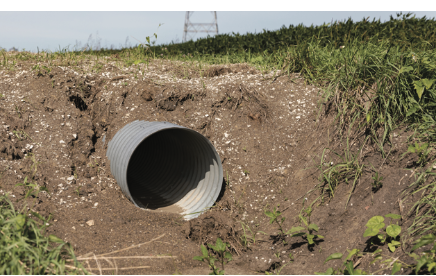
\includegraphics[width=4cm]{Hinh/CT9P1}}
\loigiai{
\begin{itemize}
\item Ống có 2 đầu hở: $\ell=k\dfrac{\lambda}{2}=\dfrac{kv}{2f}=k\dfrac{343}{2.130}\approx 1,32k\ (m)$ (với k nguyên).
\item Âm cơ bản ứng với $k=1$ nên $\ell=1,32\ m$
\end{itemize}
}
\end{ex} \haidong{20}

\loai{Tổng hợp}
\begin{ex}%book%[3P2KC-1][Loai1]
Một sóng âm có tần số 100 Hz truyền hai lần từ điểm A đến điểm B. Lần thứ nhất tốc độ truyền sóng là 330 m/s, lần thứ hai do nhiệt độ tăng nên tốc độ truyền sóng là 340 m/s. Biết rằng trong hai lần thì số bước sóng giữa hai điểm vẫn là số nguyên nhưng hơn kém nhau một bước sóng. Khoảng cách AB là
\choice
{3,4 m}
{\True 112,2 m}
{225 m}
{3,3 m}
\loigiai{
\begin{itemize}
\item Số bước sóng hơn kém nhau một $\Rightarrow$ Số bụng sóng hơn kém nhau 2 (tốc độ truyền âm nhỏ có nhiều bụng hơn)
\item Ban đầu: $100\ Hz=n. \dfrac{330}{2\ell }$ (*)
\item Lần hai: $100\ Hz=\left( n-2 \right). \dfrac{340}{2\ell }$ (**)
\item Chia từng vế (*) với (**) $\Rightarrow n = 68 \Rightarrow \ell = 112,2$ m.
\end{itemize}
}
\end{ex} \haidong{20}
\loai{Trả lời ngắn}
\begin{ex}%book
Một ống nhựa hình trụ dài $80 ~cm$, một đầu hở, một đầu kín chứa đầy một loại khí. Biết rằng khi đưa một âm thoa lại gần miệng ống và kích thích âm thoa dao động thì ống phát ra âm thanh rất to. Thay đổi tần số dao động âm kích thích thì thấy hai tần số liên tiếp làm ống phát ra âm to nhất cách nhau $430 ~Hz$. Tốc độ truyền âm trong loại khí nói trên là bao nhiêu $m/s$?\\\shortans[oly]{688}
\loigiai{
$$
\begin{aligned}
& f_{n+1}-f_{n}=(n+1) \dfrac{v}{2 l}-\dfrac{v}{2 l}=\dfrac{v}{2 l} \\
& \rightarrow \dfrac{v}{2 l}=430 \rightarrow v=430 \cdot 2 \cdot 0,8=688 ~m/s
\end{aligned}
$$
Kế quả: 688
}
\end{ex} \haidong{20}
\begin{ex}%book
Cho một ống thủy tinh hình trụ rỗng có một đầu kín và một đầu hở, dài $20 ~cm$. Bên trong ống chứa khí với tốc độ truyền âm là $350 ~m/s$. Đưa một âm thoa lại gần miệng ống và kích thích âm thoa dao động. Tần số thấp thứ ba của âm thoa để ống khí phát ra âm to nhất bằng bao nhiêu $kHz$ (làm tròn kết quả đến chữ số hàng phần trăm)?
\shortans[oly]{2,19}
\loigiai{
\begin{itemize}
\item 
Vì ống thủy tinh hình trụ rỗng có một đầu kín và một đầu hở nên
$$
f_{n}=(2 n+1) \dfrac{v}{4 \ell}
$$
\item Tần số thấp thứ ba của âm thoa để ống khí phát ra âm to nhất
$$
f_3=(2.2+1) \dfrac{v}{4 \ell}=\dfrac{5 v}{4 \ell}=\dfrac{5.350}{4.0,2}=2187,5 ~Hz=2,1875\ kHz
$$
\item Vì kết quả lấy đến 3 chữ số có nghĩa nên $f_3=2,19$
\end{itemize}
}
\end{ex} \haidong{20}
\begin{ex}%book%[3P2G6-2][Loai1]
Trong hiện tượng giao thoa sóng nước, hai nguồn dao động theo phương vuông góc với mặt nước, cùng biên độ, cùng pha, cùng tần số được đặt tại hai điểm $S_1$ và $S_2$ cách nhau 10 cm. Xét các điểm trên mặt nước thuộc đường tròn tâm $S_1$, bán kính $S_1S_2$, điểm mà phần tử tại đó dao động với biên độ cực đại cách điểm $S_2$ một đoạn ngắn nhất và xa nhất lần lượt là a và b. Cho biết $b - a = 12$ cm. Số điểm dao động với biên độ cực tiểu trên đoạn thẳng nối hai nguồn là
\choice
{2}
{3}
{\True 4}
{5}
\loigiai{
\immini{\begin{itemize}
\item Gọi N và M lần lượt là điểm dao động biên độ cực đại gần và xa $S_2$ nhất, dĩ nhiên 2 điểm này thuộc dãy cực đại ngoài cùng $k_{cd}(max)$ =$\left[ \dfrac{S_1S_2}{\lambda } \right]$\\
$\Rightarrow NS_1 - NS_2 = \left[ \dfrac{S_1S_2}{\lambda } \right].\lambda$ hay $10 - a =\left[ \dfrac{S_1S_2}{\lambda } \right]$.$\lambda \quad (*)$\\
và $MS_2 - MS_1 =  \left[ \dfrac{S_1S_2}{\lambda } \right]$.$\lambda$ hay b - 10 =$\left[ \dfrac{S_1S_2}{\lambda } \right]$.$\lambda \quad (**)$
\item Cộng từng vế (*) và (**) $\Rightarrow$ b - a = 2$\left[ \dfrac{S_1S_2}{\lambda } \right].\lambda \Rightarrow \left[ \dfrac{10}{\lambda } \right]=\dfrac{6}{\lambda } \in  Z\Rightarrow \lambda = 1$ cm hoặc 2 cm hoặc 3 cm hoặc 6 cm.
\item Thấy chỉ với $\lambda = 6$ cm là thoả mãn: $\left[ \dfrac{10}{6} \right]=\dfrac{6}{6}$= 1, vậy mỗi bên trung trực chỉ có duy nhất 1 dãy cực đại.
\item Số điểm dao động với biên độ cực tiểu trên đoạn nối hai nguồn là: $\left[ \dfrac{10}{\lambda }+0,5 \right].2=4$.
\end{itemize}}{\begin{tikzpicture}[scale=0.7,thick,>=stealth']
\tkzInit[ymin=-4,ymax=4,xmin=-3.5,xmax=4]\tkzClip
\tkzDefPoints{0/0/a, 1.5/0/o, 3/0/b, 1.5/3.5/p, 1.5/-3.5/q, -0.5/3.5/y, -0.5/-3.5/y', -3/0/b', 3.5/3.5/z, 3.5/-3.5/z'}
\tkzDefShiftPoint[a](94:3){m}
\tkzDefShiftPoint[a](28:3){n}
\tkzDrawCircle[radius,dashed](a,b)
\tkzDrawSegments(a,b p,q)
\draw[blue](y) to [bend left =30](y');
\draw[blue](z) to [bend right =30](z');
\tkzDrawPoints[size=3,fill=white](a,b,o,m,n)
\node at (a)[below]{$S_1$};
\node at (b)[below right]{$S_2$};
\node at (m)[above right]{$M$};
\node at (n)[above right]{$N$};
\node at (o)[below left]{$O$};
\end{tikzpicture}}
}
\end{ex} \haidong{20}
